\chapter{Algorithms for Interconnection Protection Relays}\label{ch_3}

This chapter explores the sophisticated logic required for Interconnection Protection Relays (IPR) in modern active distribution networks. As the grid transitions toward inverter-dominated architectures, traditional protection must be augmented with adaptive methods to handle current-limited fault signatures and bidirectional power flows. Interconnection protection is crucial for the successful integration of renewable energy sources, serving as the cornerstone for a sustainable and resilient power system.

% \section{Interconnection protection requirements}

% Interconnection protection systems are engineered to ensure strict compliance with evolving grid codes. The specific requirements for a given installation vary widely, dictated by the generator's capacity, the voltage level of the Point of Interconnection (POI)—whether at distribution or sub-transmission—and the electromechanical nature of the source (induction, synchronous, or asynchronous). Furthermore, the configuration of the interconnection transformer plays a decisive role in defining the fault current path and grounding requirements.
% The architectural requirements for DG protection must reconcile two distinct, yet equally critical, perspectives:

% \subsection{The Generator Owner's Perspective}
% The primary objective of the generator owner is to safeguard the asset from internal short circuits and external abnormal conditions that could lead to catastrophic equipment damage. Utilities can impose several detrimental states on the DG, including:
% \begin{itemize}[label=\textbullet, leftmargin=2em, nosep]
%     \item \textbf{Electrical Stresses:} Over-excitation and overvoltage conditions.
%     \item \textbf{Asymmetrical Loading:} Unbalanced currents that lead to rotor heating.
%     \item \textbf{Frequency Instability:} Abnormal frequency deviations outside of the unit's stable operating range.
%     \item \textbf{Mechanical Stress:} Severe shaft torque stress resulting from utility breaker automatic reclosing, which can lead to out-of-phase synchronization.
% \end{itemize}

% \subsection{The Utility Perspective}
% The utility's mandate is the preservation of its infrastructure and the quality of service provided to other customers. The utility is primarily concerned with
% \begin{itemize}[label=\textbullet, leftmargin=2em, nosep]
%     \item \textbf{Unwanted Fault Contributions:} DG units feeding into external faults, which can exceed the interrupting rating of existing protection devices.
%     \item \textbf{Protection Scheme Degradation:} Fundamental changes to the existing coordination and sensitivity of the protection scheme due to intermediate in-feeds and bidirectional power flows.
%    \end{itemize}


% % \begin{itemize}[label=\textbullet, leftmargin=2em, nosep]
% %     \item \textbf{Coordination Stability:} Integration must not cause over-voltages or lead to the loss of existing utility relay coordination.
% %     \item \textbf{Parallel Operation:} The system must ensure immediate disconnection when it is no longer operating in parallel with the utility grid.
% %     \item \textbf{Safety Interlocks:} The DER shall not energize the utility network when the utility itself is de-energized (prevention of back-feeding).
% %     \item \textbf{Islanding Prevention:} Active and passive measures must be implemented to prevent the creation of unintentional islands.
% %     \item \textbf{Relay Standards:} All protection systems must utilize ``utility grade'' relays to ensure reliability and high-speed fault clearance.
% %     \item \textbf{Power Quality:} The DER must not inject objectionable harmonics that degrade the performance of the utility grid or connected customer equipment.
% %     \item \textbf{Synchronization:} The initiation of parallel operation must not cause a loss of synchronization or objectionable flicker in the local network[.
% %     \item \textbf{Voltage Regulation:} The DG unit must not cause over-voltages during steady-state or transient operating conditions.
% % \end{itemize}

% % The DG protection is established from the Point of Common Coupling (PCC) and the interconnection transformer.The Point of Common Coupling (PCC) is located in the substation where the Distributed Generation (DG) is interconnected with the grid. Sometimes also referred as Point of Common Connection or Point of Connection (PoC). The purpose of the interconnection protection is to protect the grid from the DG unit on the grid-side during parallel operations of the DG and the grid.  The protection can be located either on the primary side of the interconnection transformer or on the secondary side  as shown in Figure.

% \subsection{Industrial Performance Criteria} 

% Interconnection protection systems are engineered to ensure strict compliance with evolving grid codes. To maintain the integrity of the broader network, the following technical constraints must be rigorously addressed:

% \begin{itemize}[label=\textbullet, leftmargin=2em, nosep] \item \textbf{Coordination Stability:} The integration of localized sources must be managed to prevent over-voltages and ensure the continued selectivity of existing utility relay coordination. \item \textbf{Parallel Operation:} Protection logic must facilitate the immediate decoupling of the DER when it is no longer operating in parallel with the utility grid to prevent unsynchronized operation. \item \textbf{Safety Interlocks:} To protect utility personnel and infrastructure, the DER must not energize a de-energized utility network, effectively preventing hazardous back-feeding. \item \textbf{Islanding Prevention:} A robust combination of active and passive measures is required to detect and mitigate the formation of unintentional islands. \item \textbf{Relay Standards:} All protection schemes must utilize ``utility grade'' relays, ensuring the reliability and high-speed fault clearance necessary for utility-scale stability. \item \textbf{Power Quality:} The DER interface must be designed to suppress objectionable harmonics that could degrade utility performance or interfere with sensitive customer equipment. \item \textbf{Synchronization:} The initiation of parallel operation must be precisely controlled to avoid loss of synchronization or the introduction of objectionable voltage flicker into the local network. \item \textbf{Voltage Regulation:} DG units must operate within specified bounds, ensuring they do not cause over-voltages during either steady-state or transient grid conditions. \end{itemize}

% %\subsection{Compliance and Type Testing}
% %Validation procedures according to VDE and German grid codes for unit certification.

% \section{The Point of Interconnection and Protection Architecture}
% % The technical boundary for DG protection is established at the Point of Common Coupling (PCC)—alternatively referred to as the Point of Common Connection or Point of Connection (PoC). This critical node is typically situated within the substation where the DG unit interfaces with the utility infrastructure.

% % The overarching objective of IPR is the protection of the utility grid from potential DG-side disturbances during parallel operation. Depending on the system's voltage level and the specific grounding requirements of the plant, the protective elements may be strategically located on either the primary or the secondary side of the interconnection transformer. This placement is vital for ensuring that the relay has the necessary visibility into both internal plant faults and external grid disturbances

% The Point of Interconnection (POI), also known as the Point of Common Coupling (PCC), is the critical interface where the generator facility connects to the utility grid.The protection architecture at this location must provide visible isolation, overcurrent protection, and the sensing necessary for the IPR functions.A typical protection architecture includes:
% Isolation Switch: A manually operated, lockable switch providing a visible break for utility personnel.
% High-Side Interrupting Device: A circuit breaker or recloser capable of interrupting the maximum available short-circuit current from both the grid and the DG.
% Interconnection Transformer: The winding configuration (e.g., Delta-Wye) is crucial, as it determines the zero-sequence current path. Utilities often specify configurations that prevent the DG from becoming a ground source for grid faults, which would otherwise desensitize ground overcurrent relays.

% IPR Sensing: Voltage and current transformers (VT/CT) must be placed to monitor both the grid and the DG side of the PCC to facilitate synchronization and detect islanding.


% \begin{figure}[!h]
% \centering{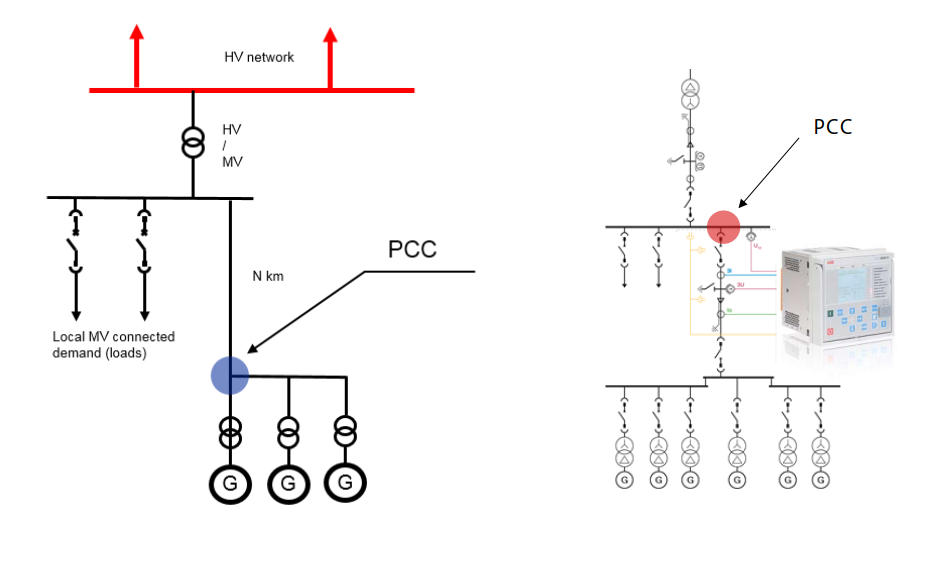
\includegraphics[width=0.75\textwidth]{images/chapter_3/PCC1.png}}
% \caption{Application of IPR at the PCC\label{Fig1}}
% \end{figure}


% \subsubsection{Factors Influencing Interconnection Protection} 

% \subsubsection{Technical Boundary:}
% Defining the PCC as the critical substation interface.
% \subsubsection{Protection Infrastructure:}
% Role of isolation switches, circuit breakers, and sensing units (VTs/CTs).
% \subsubsection{ Transformer Winding Influence:}
% How YNd or Dyn configurations dictate zero-sequence current paths and grounding requirements.
% The choice of transformer plays an important role in the DG connection with the utility.  All connections have advantages and disadvantages that need to be considered by the utility and distributed generation owner.  The type of ground connection is classified as: solidly grounded, ungrounded or grounded through grounding impedance.  

% \subsubsection{Types of DG} 
% Generators can be divided into traditional and non-traditional generators. The inverters are classified by two types: line-commutated (thyristor based) and self-commutated inverters (IGBT or MOSFET based). Normally DGs are operated in a constant power and constant power factor control mode which makes it improbable that precise balance will occur when the utility is lost and an unintentional island formed. Inverters can also be used to implement active islanding detection schemes.  






\section{Interconnection Protection Relay}
The IPR is a multi-function digital device that integrates various protective functions (ANSI codes) into a single hardware platform. Modern IPRs must process high-frequency sampling data to implement complex algorithms while maintaining interoperability through protocols like IEC 61850, DNP3, or Modbus.




\begin{figure}[t!]
	\centering
	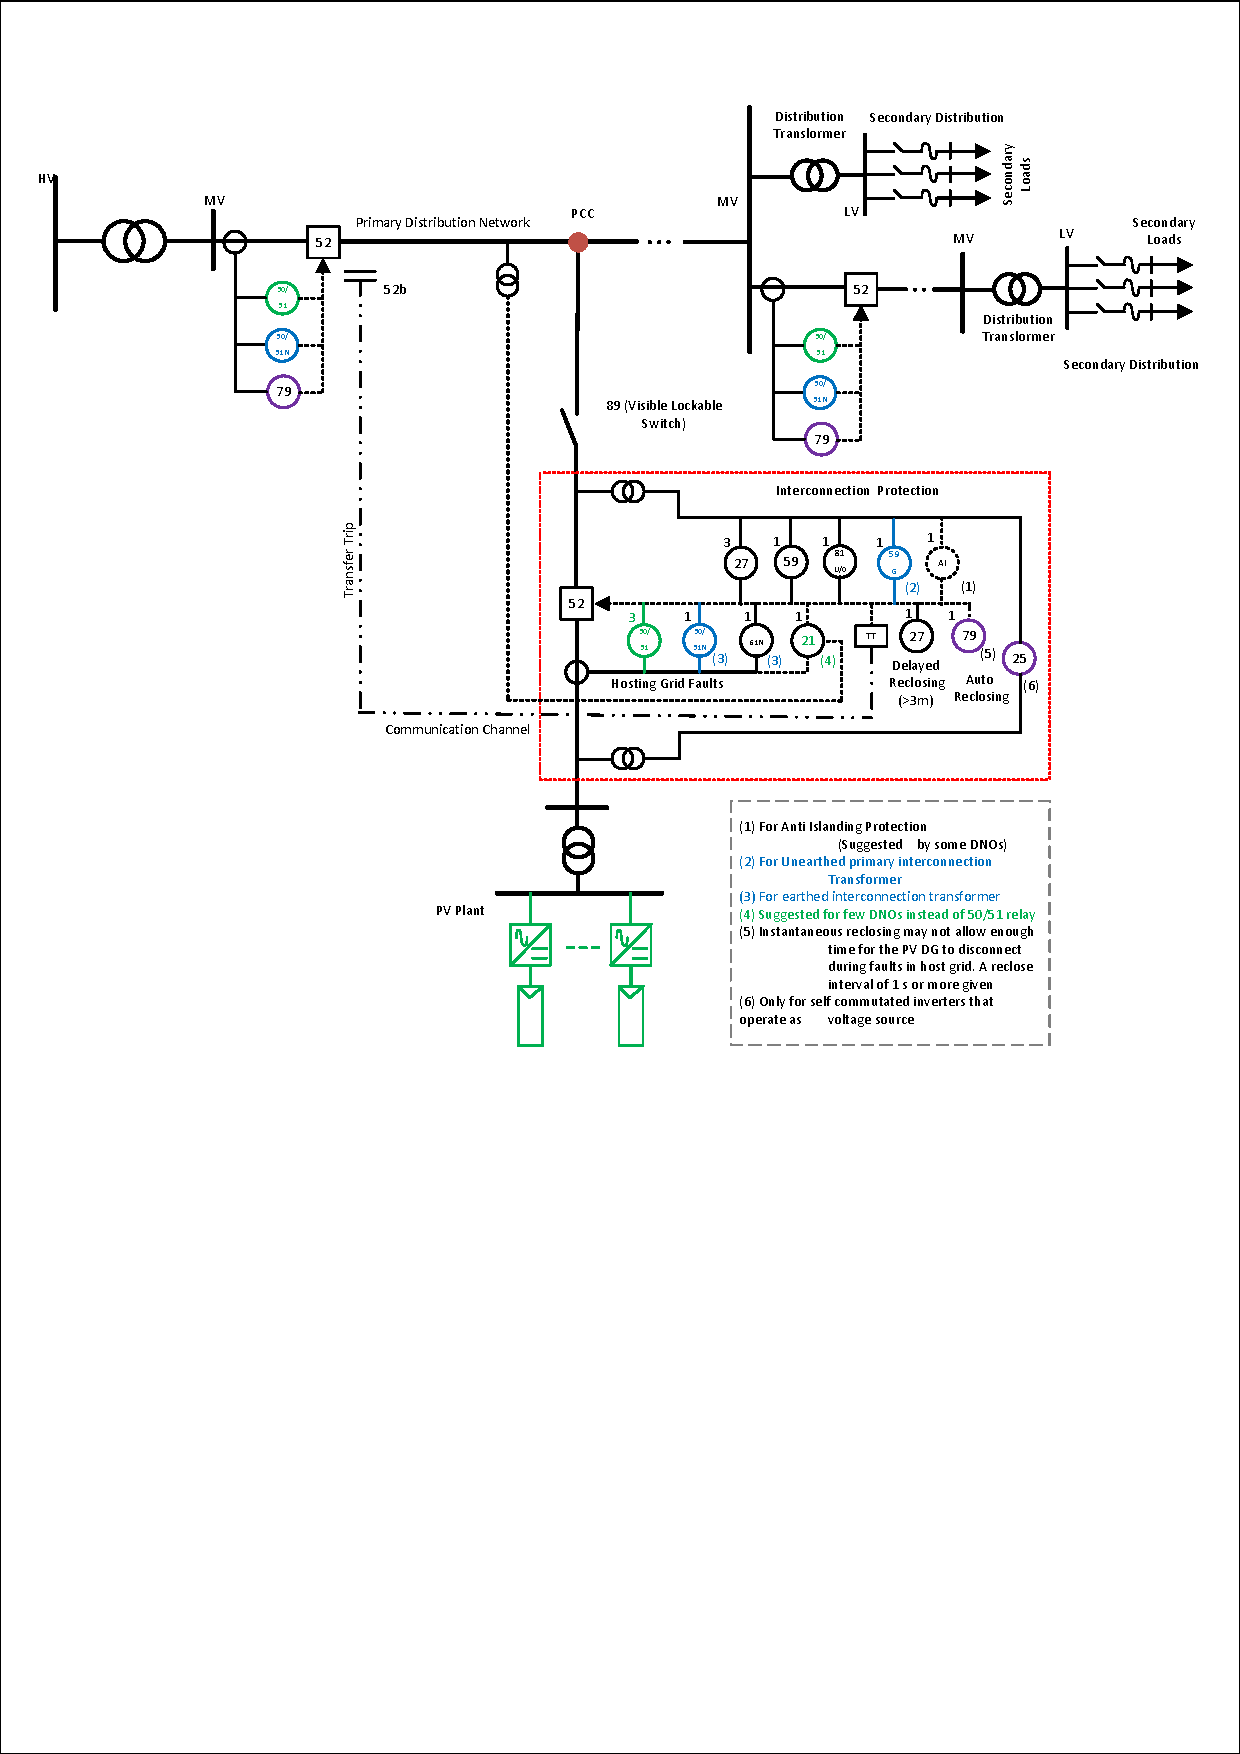
\includegraphics[page=1, scale=0.7, trim={10 320 10 10}, clip]{images/chapter_3/eluva1.pdf}
 
	\caption{Interconnection protection using multi-function relays for a PV plant connected to MV distribution network}
	\label{Fig2}
\end{figure}
% %%%%%%%%%%%%%%%%%%%%%%%%%%%%%%%%%%%%%%%%%%%%%%%%%%%
% \begin{figure}[h]
%     \centering
%     % \includestandalone strips the preamble of the child file and renders the TikZ natively
%     \includestandalone{Z_Final_Thesis_figures/ch4_IPR/c4_1_sch_adaptive_logic}
%     \caption{Adaptive LVRT decision logic for grid-tied inverter systems.}
%     \label{fig:c4_1_adaptive_logic}
% \end{figure}


\begin{figure}[h]
    \centering
    % \includegraphics pulls the PDF vector directly
    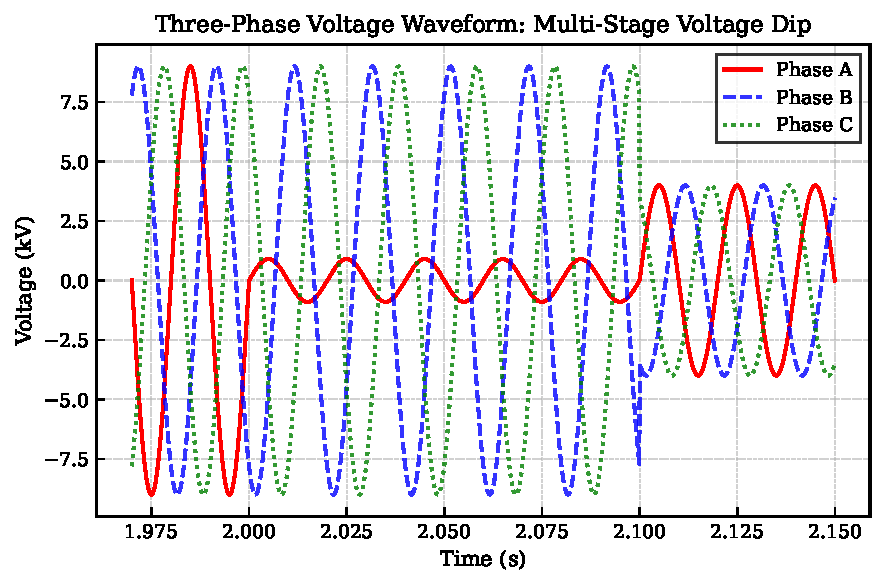
\includegraphics[width=0.8\textwidth]{Z_Final_Thesis_figures/ch4_IPR/c4_3_plt_multistage_voltage_dip.pdf}
    \caption{Three-phase voltage waveform demonstrating a multi-stage voltage dip during SLG fault transition.}
    \label{fig:c4_3_multistage_dip}
\end{figure}
 %%%%%%%%%%%%%%%%%%%%%%%%%%%%%%%%%%%%%%%%%%%%%%%%%%

\begin{itemize}[label=\textbullet, leftmargin=2em, nosep]
    \item \textbf{Anti-Islanding (ANSI 78/81R):} In addition to passive methods (OVP/UVP and OFP/UFP), active techniques such as \textit{Active Frequency Drift} (AFD) or \textit{Sandia Frequency Shift} (SFS) are implemented in the inverter control to destabilize the voltage/frequency if the utility is lost, forcing the relay to trip.
    \item \textbf{Reverse Power (ANSI 32):} This element prevents the DER from feeding power back into the utility if the interconnection agreement is for "Zero Export." It is also critical for protecting local synchronous generators from motoring.
    \item \textbf{Over/Under-Voltage (ANSI 59/27):} These elements are coordinated with the LVRT/HVRT curves mandated by IEEE 1547. Under-voltage elements must distinguish between a temporary grid fault and a permanent loss of utility.
    \item \textbf{Over/Under-Frequency (ANSI 81O/U):} Since microgrids have low inertia, frequency deviations occur rapidly ($\text{high } df/dt$). Rate of Change of Frequency (ROCOF) relays are often employed for faster islanding detection.
\end{itemize}


% Requires: \usepackage{booktabs}
\begin{table}[h!]
    \centering
    \caption{Multi functional relay functions}
    \label{tab:placeholder_label}
    \begin{tabular}{lll}
        \toprule
        ANSI Function & Designation & Operational Requirement \\
        \midrule
        27    & Undervoltage         & Must ride through Category III sags to 0.05 p.u. \\
        59    & Overvoltage          & Detects surges from load rejection or islanding \\
        81U/O & Under/Over Frequency & Frequency-Watt drooping for grid stability \\
        32    & Reverse Power        & Directional power flow monitoring at PCC \\
        25    & Sync-Check           & Prevents out-of-phase reclosing \\
        \bottomrule
    \end{tabular}
\end{table}
\subsection{IPR for Solar Plants}
IPR for Solar PV plants must account for the source's inertialess nature. Unlike rotating machines, Solar PV fault contribution is governed by the MPPT and current-limiting algorithms of the inverter. IPRs in these plants primarily focus on:
\begin{itemize}
    \item \textbf{DC Offset and Harmonic Monitoring:} Detecting DC injection into the AC grid, which can saturate distribution transformers.
    \item \textbf{Phase Jump Detection:} Monitoring sudden shifts in the voltage phase angle ($\Delta\theta$) that indicate a change in the network's Short Circuit Ratio (SCR).
\end{itemize}

\subsection{IPR for Wind Plants}
Protection for wind plants varies significantly by turbine type. Type III (DFIG) plants require sophisticated IPRs that can handle the asymmetrical fault currents produced when the rotor "crowbar" is engaged. Type IV wind plants share similarities with Solar PV but often include larger-scale STATCOM functionalities for reactive power support. The IPR must ensure that the "Negative Sequence Overcurrent" (ANSI 46) does not cause nuisance tripping during external unbalanced faults while still protecting the generator from internal asymmetries.

% \section{Advanced protection schemes- proposed logics} 

\section{The fault phase selection logic}
Fault phase selection is critical for modern numerical relays to ensure correct distance reach ($Z$) and to enable Single-Pole Tripping (SPT). In IBR-dominated systems, traditional delta-current ($\Delta I$) or sequence-component-based selection logic often fails due to:
\begin{enumerate}
    \item \textbf{Negative Sequence Suppression:} Many inverters suppress $I_2$, making L-G and L-L fault identification difficult using sequence ratios ($I_2/I_1$).
    \item \textbf{Voltage-Current Phase Displacement:} $I_q$ injection during faults shifts the current's phase, potentially leading to the selection of the wrong phase loop in distance elements.
\end{enumerate}
Modern logic now employs Incremental Quantity Analysis and Superimposed Complex Power ($\Delta S$) to accurately identify the faulted phase even under current-limited conditions.

Various power system events can cause significant voltage variations.~The designed expert system for fault phase selection logic must classify these events into fault event and non-fault events (such as transformer saturation, starting of motor, or interruption).~Different algorithms have been studied to identify suitable methods for voltage sag characterization.~A generalized method for classifying unbalanced sags using symmetrical components was introduced in .~Two parameters, characteristic voltage (CV) and positive negative factor (PNF), provide a better characterization of a single-event voltage sag.~The parameter CV can be used as a single-phasor equivalent for three-phase voltages.

A method for characterizing voltage dips based on the space phasor model (SPM) estimated from three-phase voltages was introduced in.~The SPM in the complex plane holds the signature of voltage sag.~The projection of the SPM in a complex plane is a circle for a voltage sag owing to balanced faults and ellipses for unbalanced faults.~The voltage sag parameters can be estimated from the ellipse parameters , in which CV is quantitatively equivalent to the minor axis length of the ellipse, and PNF is equivalent to the major axis length of the ellipse.~This principle was used to design the EVPM.~Three-phase-to-neutral-voltages were continuously monitored at the IPR terminals.~EVPM estimates the SPM from the measured instantaneous three-phase voltages .~The voltage sag parameters, CV and PNF were estimated from the ellipse major and minor axis lengths.~The fault types were estimated based on the tilt of the major axis of an ellipse.

For illustration, the waveforms of a multi-stage voltage sag event are shown in Figure \ref{multisagdip}.~A single-phase to ground-fault event followed by a three-phase fault event was examined.~A plot of the three-phase-to-neutral voltages is shown in Figure~\ref{multisagdip}~(a).~The SPM was estimated from the three-phase voltages.~The variation of SPM magnitude and its RMS value is given in Figure~\ref{multisagdip}~(b)~The multi-stage voltage dip events can be classified into,~pre-fault,~fault and post-fault events.~Voltage dip characteristics were estimated as single-event characteristics by dividing them into event segments.~The estimated SPM is shown in Figure~\ref{multisagdip}~(c) and the segments are shown in Figure~\ref{multisagdip}~(d).




\subsection{Mathematical Foundation:} 

Space Phasor Model (SPM) derivation using the Clarke Transformation.

Voltage sags are classified into types A, C, and D types.~The phasor representations of these sag types and their corresponding SPM plots in the polar plane are shown in Figure~\ref{multisagdip}.~The type A sag has an equal voltage dip in all phases which can be caused by a three-phase fault or a non-fault event such as the switching of a large load.~Type C is characterized by a large dip in the two phases and a slight dip in the third phase.~This was caused by the two-phase faults.~These C-type dips were further classified into $C_a$, $C_b$, and $C_c$ based on the phase with the lowest dip.~Type D represents single-phase faults with large dips in a single phase.~The D-type dips were classified into $D_a$, $D_b$, and $D_c$ based on the phase with the most significant dip.~The voltage dips were characterized by CV, PNF, and dip-type (DT).


\begin{figure}[t!]
    \centering{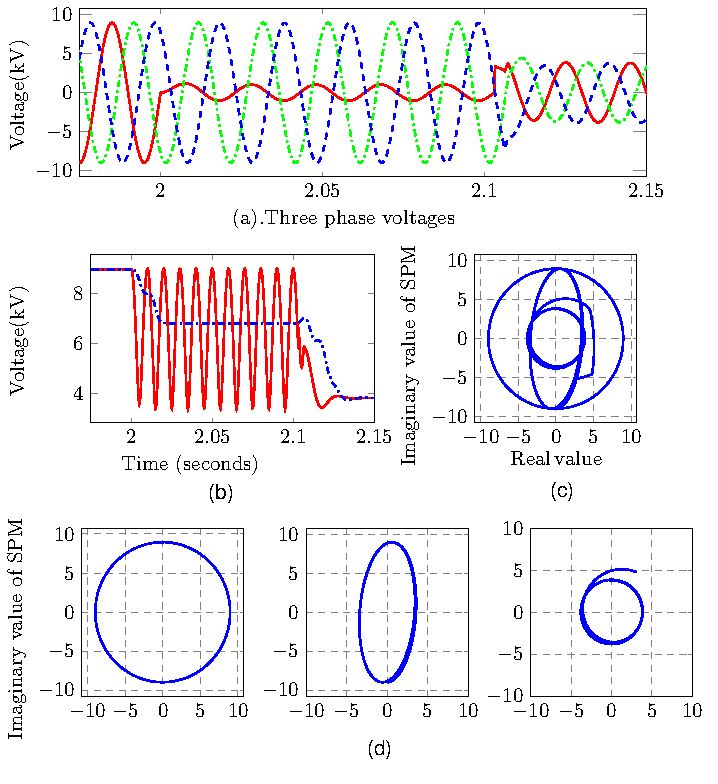
\includegraphics[page=1,  scale=1, trim={0 0 00 0}, clip]{images/chapter_3/eluva3.pdf}}
	\caption{Multi-stage voltage dip and polar plot of SPM.}
	\label{multisagdip}
\end{figure}


\begin{figure}[t!]
\centering
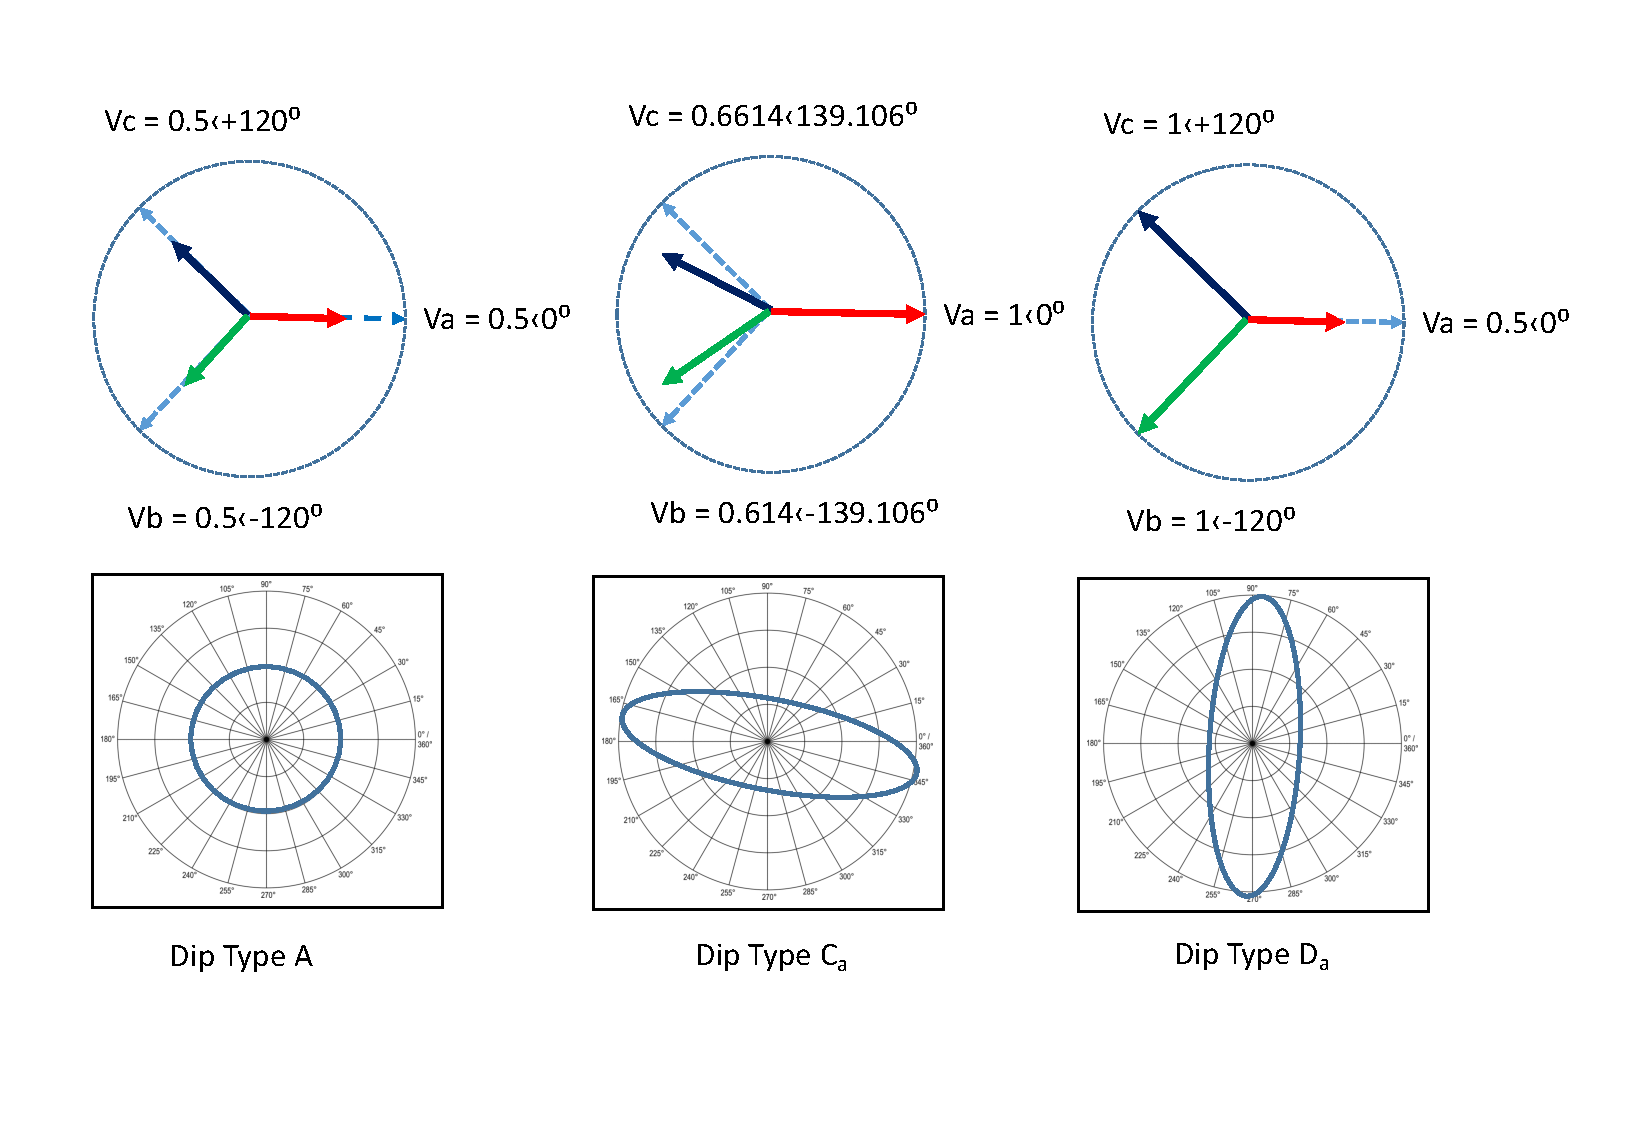
\includegraphics[scale=0.35,trim={1.5cm 1.5cm 1.2cm 1.2cm},clip]{images/chapter_3/eluva5.pdf}
\caption{Voltage sags  (A, C, and D types) and their corresponding SPM plot in polar plane.}
\label{acddips}
\end{figure}


The fundamental components for three phase to neutral voltages can be represented as,
\begin{align}
v_{a}{(t)}&=\sqrt{2}~\times~ K_{1}~\times~V_{a}~Sin(wt+\phi_{1})\\
v_{b}{(t)}&=\sqrt{2}~\times~ K_{2}~\times~V_{b}~Sin(wt-120+\phi_{2})\\
v_{c}{(t)}&=\sqrt{2}~ \times~K_{3}~\times~V_{c}~Sin(wt+120+\phi_{3}) .
\end{align}
Where $V_{a}$,$V_{b}$, and $V_{c}$ are the RMS values of the three-phase voltage. The scaling factors K1,K2 and K3 are equal to 1 and the angle changes $\phi_{1}$,$\phi_{2}$, and $\phi_{3} $ are equal to 0, for a three-phase balanced healthy system during nominal operation. The fault cases are represented by changes in the values of the scaling factors K1,K2, and K3 between 0 and 1 based on the fault severity and the vector shifts  $\phi_{1}$ , $ \phi_{2}$, and $\phi_{3}$  between 0 and 120.

The Clarke Transformation of three phase voltage is evaluated as 
\begin{equation}
\begin{bmatrix}
x_{\alpha}(t)\\\\
x_{\beta}(t)\\
\end{bmatrix}=\frac{2}{3}
\begin{bmatrix}
1&-\frac{1}{2}&-\frac{1}{2}\\\\
0&\frac{\sqrt{3}}{2}&-\frac{\sqrt{3}}{2}\\
\end{bmatrix}
\begin{bmatrix}
v_{a}(t)\\\\
v_{b}(t)\\\\
v_{c}(t)\\
\end{bmatrix}.\\
\end{equation}

The SPM for three-phase voltages, $v_{a}$,~ $v_{b}$, and $v_{c}$ is obtained from the Clarke transformation as follows:-
\begin{equation}
SPM =  \vec{s}(t) = x_{\alpha}(t) + j~x_{\beta}(t).
\end{equation}
Which can be derived in terms of three phase voltages as
\begin{equation}\label{spmequation}
SPM = \vec{s}(t) =\frac{2}{3}[v_{a}{(t)}+\alpha \times  v_{b}{(t)}+\alpha^{2} \times v_{c}{(t)}]
\end{equation}
where $\alpha = e^\frac{j2\pi}{3}$.


The shape of the SPM in a complex plane is circular or elliptical.~The generalized equation of an ellipse in terms of Cartesian coordinates is defined as,
\begin{equation}
	\text{a}x^{2} + \text{b}xy + \text{c}y^{2} + \text{d}x + \text{e}y - \text{f} = 0.
\end{equation}

The SPM was estimated for instantaneous-three phase voltages  $\text{v}_{a}$,$\text{v}_{b}$, and $\text{v}_{c}$ measured at the IPR terminals.~The general ellipse model for the instantaneous values of SPM = ($x_\text{i} + \text{j}~ y_\text{i}$) can be written as,


\begin{equation}
	h(\theta_\text{i})=\text{a}x_{\text{i}}^{2} + \text{b}x_\text{i}y_\text{i} + \text{c}y_{\text{i}}^{2} + \text{d}x_{\text{i}} + \text{e}y_{\text{i}} = 1.
\end{equation}

\subsection{Real-time Extraction:} 

Direct Least Squares Estimation for tracking elliptical locus eccentricity. The ellipse parameters are calculated by finding the best fit to a hypothetical ellipse represented by the generalized equation discussed above using the direct least square estimation introduced in 
\cite{Fitzgibbon}. The algorithm is robust to noise and requires less memory to perform operations and less time-consuming computations.



\begin{equation}
	f(\theta)=\sum_{i=1}^{n} {(\text{a}x_{\text{i}}^{2} + \text{b}x_\text{i}y_\text{i} + \text{c}y_{\text{i}}^{2} + \text{d}x_{\text{i}} + \text{e}y_{\text{i}} - 1)^2} 
\end{equation}
where n is the number of samples in the moving window.

The cost function in vectorized form can be expressed as

\begin{equation}
	f(\theta)=(\text{X} \theta - \text{N})^{\text{T}} (\text{X} \theta - \text{N})
\end{equation}
where
\begin{equation}
	\begin{bmatrix}
		\text{X} 
		
	\end{bmatrix}=
	\begin{bmatrix}
		x_{\text{i}}^{2} & x_\text{i}y_\text{i} & y_{\text{i}}^{2} & x_{\text{i}}&y_{\text{i}}\\
		\vdots&\vdots&\vdots&\vdots&\vdots\\
		x_{\text{i}}^{2} & x_\text{i}y_\text{i} & y_{\text{i}}^{2} & x_{\text{i}}&y_{\text{i}}
	\end{bmatrix}
\end{equation}\label{equvector}
and,
\begin{equation}
	\begin{bmatrix}
		\text{N} 
		
	\end{bmatrix}=
	\begin{bmatrix}
		1\\
		\vdots\\
		1
	\end{bmatrix}_{n=1}.
\end{equation}\\
For estimating the ellipse parameters f($\theta$) is minimized with respect to $\theta$.
\begin{equation} 
	\frac{\partial~f}{\partial~\theta}=0 ~ ; ~\nabla_{\theta} f=0 .
\end{equation} 

% \subsection{Signature Characterization:} 

Mapping CV, PNF, and Tilt Angle ($\phi$) to fault types.
\begin{table*}[h!]
	\centering
	\caption{Estimated values for CV, PNF and Inclination angle for voltage sags 0.5PU and 0.88PU for various fault types.}
	\label{tablecvpnf}
	\begin{tabular}{c|ccccc|ccccc|c}\hline
		&\multicolumn{5}{c|}{Voltage Sag=0.5 PU} & \multicolumn{5}{c|}{Voltage Sag=0.88 PU} \\ \hline
		Fault Type & Va & Vb & Vc & CV & PNF & Va & Vb & Vc & CV & PNF & Theta($Degree$)\\ \hline
		A & 0.5 & 0.5 & 0.5 & 0.5 & 0.5 &0.88 & 0.88 & 0.88 & 0.88 & 0.88 & 0  \\ &&&&&&&&&&&\\
		$D_a$&0.5 & 1 & 1 & 0.66 & ~1 &0.88 & 1 & 1 & 0.92 & 1 & 60-90  \\ 
		$D_b$&1 & 0.5 & 1 & 0.66 & ~1 & 1 & 0.88 & 1 & 0.92 & 1 & 0-30 \\
		$D_c$&1 & 1 & 0.5 & 0.66 & ~1 & 1 & 1 &0.88 & 0.92 & 1 &120-150 \\&&&&&&&&&&&\\
		$C_a$&1 & 0.66 & 0.66 & 0.5 & 1& 1 & 0.91& 0.91 & 0.88 & 1 & 150-180 \\ 
		$C_b$&0.66 & 1 & 0.66 & 0.5 & 1& 0.91 & 1 & 0.91 & 0.88 & 1 & 90 -120  \\ 
		$C_c$&0.66 & 0.66 & 1 & 0.5 & 1 & 0.91 & 0.91 & 1 & 0.88 & 1 & 30-60\\&&&&&&&&&&&\\
		$E_a$&1 & 0.5 & 0.5 & 0.5 & 0.83 & 1 & 0.88 & 0.88 & 0.88 & 0.96 & 60-90 \\ 
		$E_b$&0.5 & 1 & 0.5 & 0.5 & 0.83 & 0.88 & 1 & 0.88 & 0.88 & 0.96 & 0-30 \\
		$E_c$&0.5 & 0.5 & 1 & 0.5 & 0.83 & 0.88 & 0.88 & 1 & 0.88 & 0.96 & 120-150 \\
		 \hline
	\end{tabular}
\end{table*}



\begin{figure*}[t!]
\centering
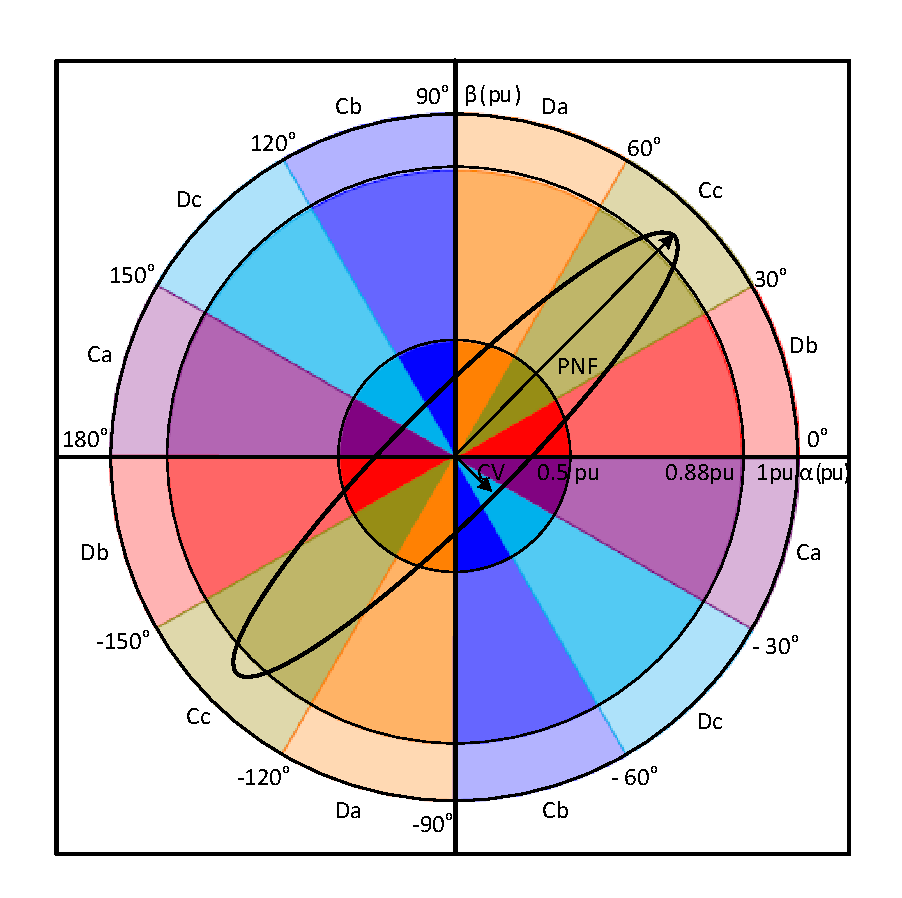
\includegraphics[scale=0.6]{images/chapter_3/eluva7.pdf}
\caption{Undervoltage protection setting characteristics chart for EVPM with loccus of a SLG fault.}
\label{Fig2}
\end{figure*}




\section{Enhanced Voltage Protection Module (EVPM)}

% \subsection{EVPM}

The Enhanced Voltage Protection Module (EVPM) is a sophisticated technique designed to maintain protection coordination in active networks where short-circuit levels are highly variable. Standard coordination fails because the "seen" impedance or current depends on whether the system is grid-connected or islanded.


\begin{figure}[t!]
	\centering
	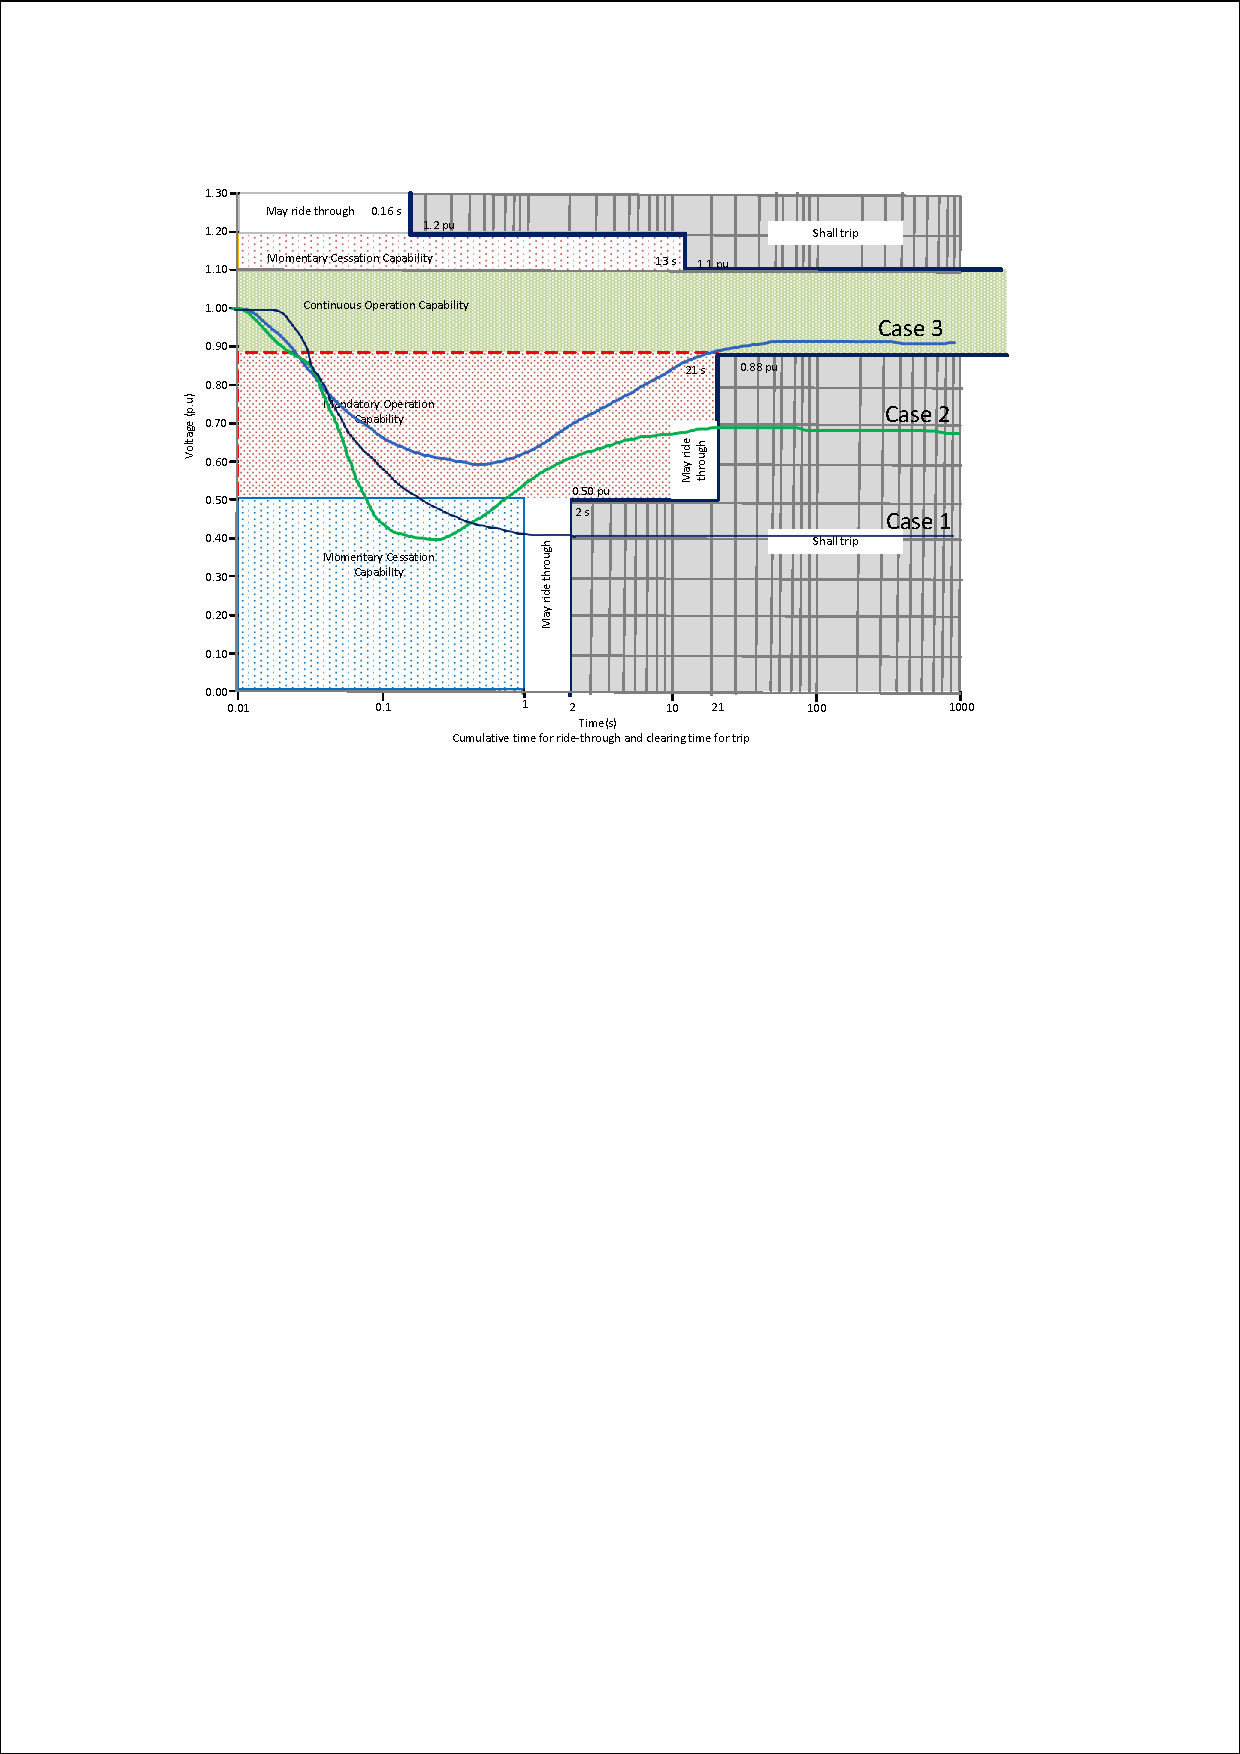
\includegraphics[scale=1, trim={80 480 100 70}, clip]{images/chapter_3/LVRT_IEEE.pdf}
	\caption{An estimation of tripping time for various voltage dips based on LVRT requirement for Category III DER according to IEEE 1547 - 2018 standard}.
	\label{lvrtcategory3}
\end{figure}



Segmented Sag Analysis: Using the EVPM to detect upstream recloser "dead time" and persistent faults to override LVRT mandates.

Proposed Enhancements for Coordination:

\begin{itemize}
    \item \textbf{Dynamic Thresholding:} Adjusting the EVPM calculation based on the specific equipment at the fault location (Generator, Transformer, or Busbar) to account for localized physical component characteristics.
    \item \textbf{Imbalance Compensation:} Integrating logic that accounts for faults categorized by phase imbalance to prevent nuisance tripping during unsymmetrical grid disturbances.
    \item \textbf{Initiation Source Weighting:} Incorporating the cause of initiation—whether natural (lightning), human-induced, or equipment aging—to prioritize trip signals during critical grid disturbances.
    \item \textbf{Nature of Connection Logic:} Enhancing the EVPM to adapt its sensitivity based on whether the fault involves ground contact (Grounded vs. Ungrounded), ensuring selectivity remains robust across all fault topologies.
    \end{itemize}




As discussed in the previous section, the use of conventional undervoltage relays (27) as in multi-function IPR, poses challenges.~To overcome this issue, the proposed EVPM logic uses an expert algorithm
for voltage sag characterization to coordinate precisely with reclosing relays in the host network and ensure instantaneous isolation of DG sources for faults in the host DN.~Fault-induced voltage sags consist of multiple stages of magnitude before they return to the nominal value.~The inception of the fault and the subsequent operation of the recloser in the host DN can be sensed as a multi-stage voltage dip at the IPR terminals.~These multi-stage voltage dips are characterized after segmenting the measured voltage into several events (refer to Figure~\ref{multisagdip}).


 A fault in the host network can be detected based on the voltage sag estimation using undervoltage functions\cite{pnnlgov}.
The conventional undervoltage functions (27) used in multi-function 
IPR calculate the root mean square (RMS) of three-phase voltages to
estimate the residual voltage and its duration for characterizing
undervoltage events\cite{pnnlgov}. Various studies have concluded that a variety of power system events (fault or non-fault events such as islanding, transformer saturation, and motor starting) cause significant voltage variations in large parts of the network~\cite{bollen2000understanding}.~Therefore, it is challenging to differentiate between various voltage sag events based on residual voltage and duration.~To overcome these issues a method based on voltage sag characterization at the PCC is proposed in the present work.



Another purpose of voltage sag characterization is to
coordinate with the reclosing relays (79) in the host network.~In
general, overhead radial MV distribution feeders use line
reclosers to clear temporary faults.~Following a fault, the DG sources connected to the network must be removed to ensure a successful reclosing.~In common practice, for DN with high penetration of DG sources, the reclosing attempt has to be delayed (0.3s used for fast reclosing is delayed upto~1s) to ensure the isolation of DGs ~\cite{pnnlgov}.~This causes a significant increase of power interruption time, in distribution networks with DG sources.~Figure \ref {flowchartref} shows an estimation of tripping time for various voltage dips based on LVRT requirement for Category III DER according to IEEE 1547-2018 standard.~The tripping time of the DG is determined based on the RMS values of the voltages.~Shall-trip voltage default settings for Category III DER based on IEEE 1547-2018 standard is given in table~\ref {LowvolttriptimesIEEE}.~The variations in trip times for Case~I~, Case~II, and Case~III sag events are shown in~Figure~\ref {lvrtcategory3}.~The proposed EVPM utilizes voltage sag characterization to detect must trip conditions, and it is estimated without any time delay.~The following section explains the proposed method.


\begin{figure}[t!]
    \centering
    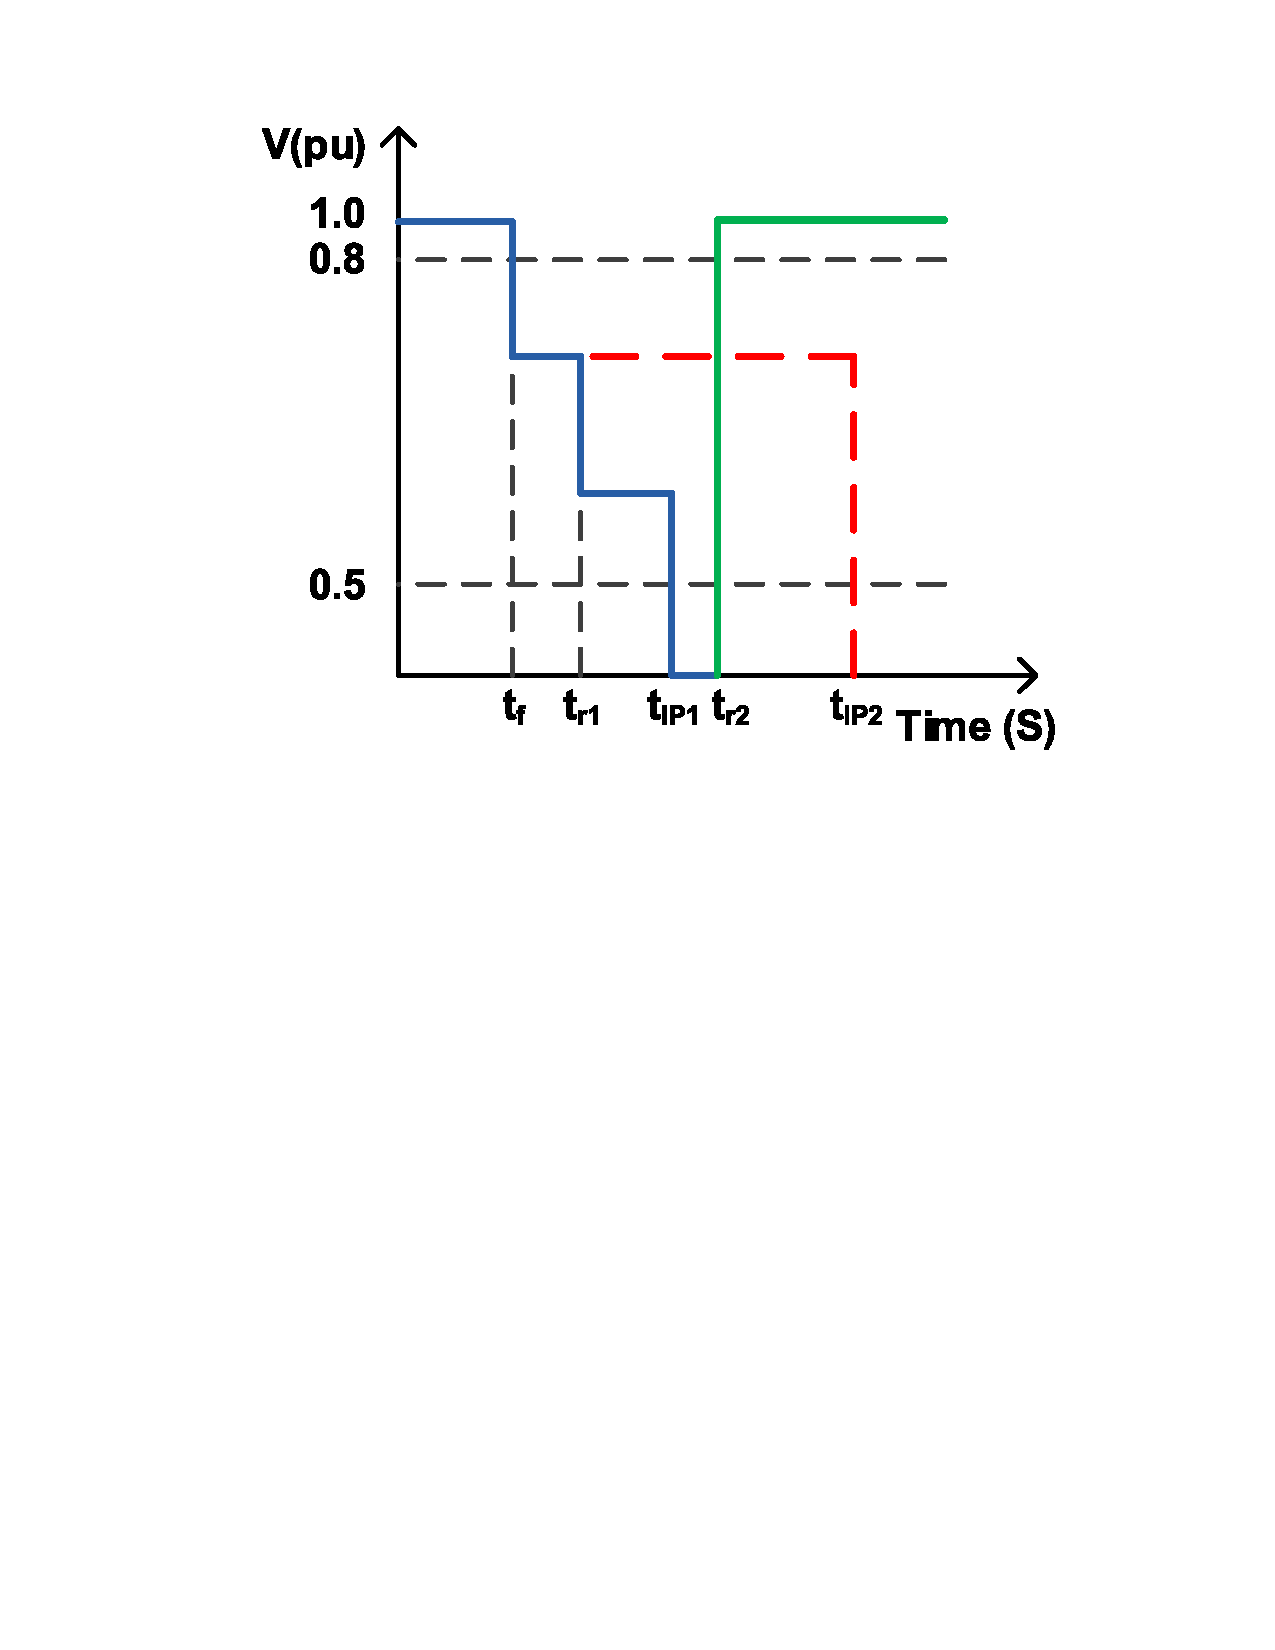
\includegraphics[page=1,  scale=.8, trim={100 420 100 50}, clip]{images/chapter_3/eluva4.pdf}
	\caption{Operational time of EVPM after a multi-stage voltage sag.}
	\label{relaytriptimes}
\end{figure}



The EVPM algorithm coordinates with line reclosers in MV radial distribution networks.~The operational time coordination of the proposed EVPM with an upstream recloser is illustrated in Figure~\ref{relaytriptimes}.~For a fault occurring at time $t_f$, a voltage dip was sensed at the IPR terminals.~If an upstream reclosing relay operates at time $t_{r1}$, a second dip in the voltage is sensed at the IPR terminals.~If the fault is fed by the PV DG, EVPM detects a persisting fault, and the tripping command is given at time $t_{Ip1}$.~The recloser can be successfully reclosed in a very short time $t_{r2}$.~If the IPR seeing undervoltage dip operates as a conventional undervoltage relay with operating time as defined in the standards, it would have operated with a much delayed time $t_{Ip2}$.


\begin{figure*}[t!]
\centering
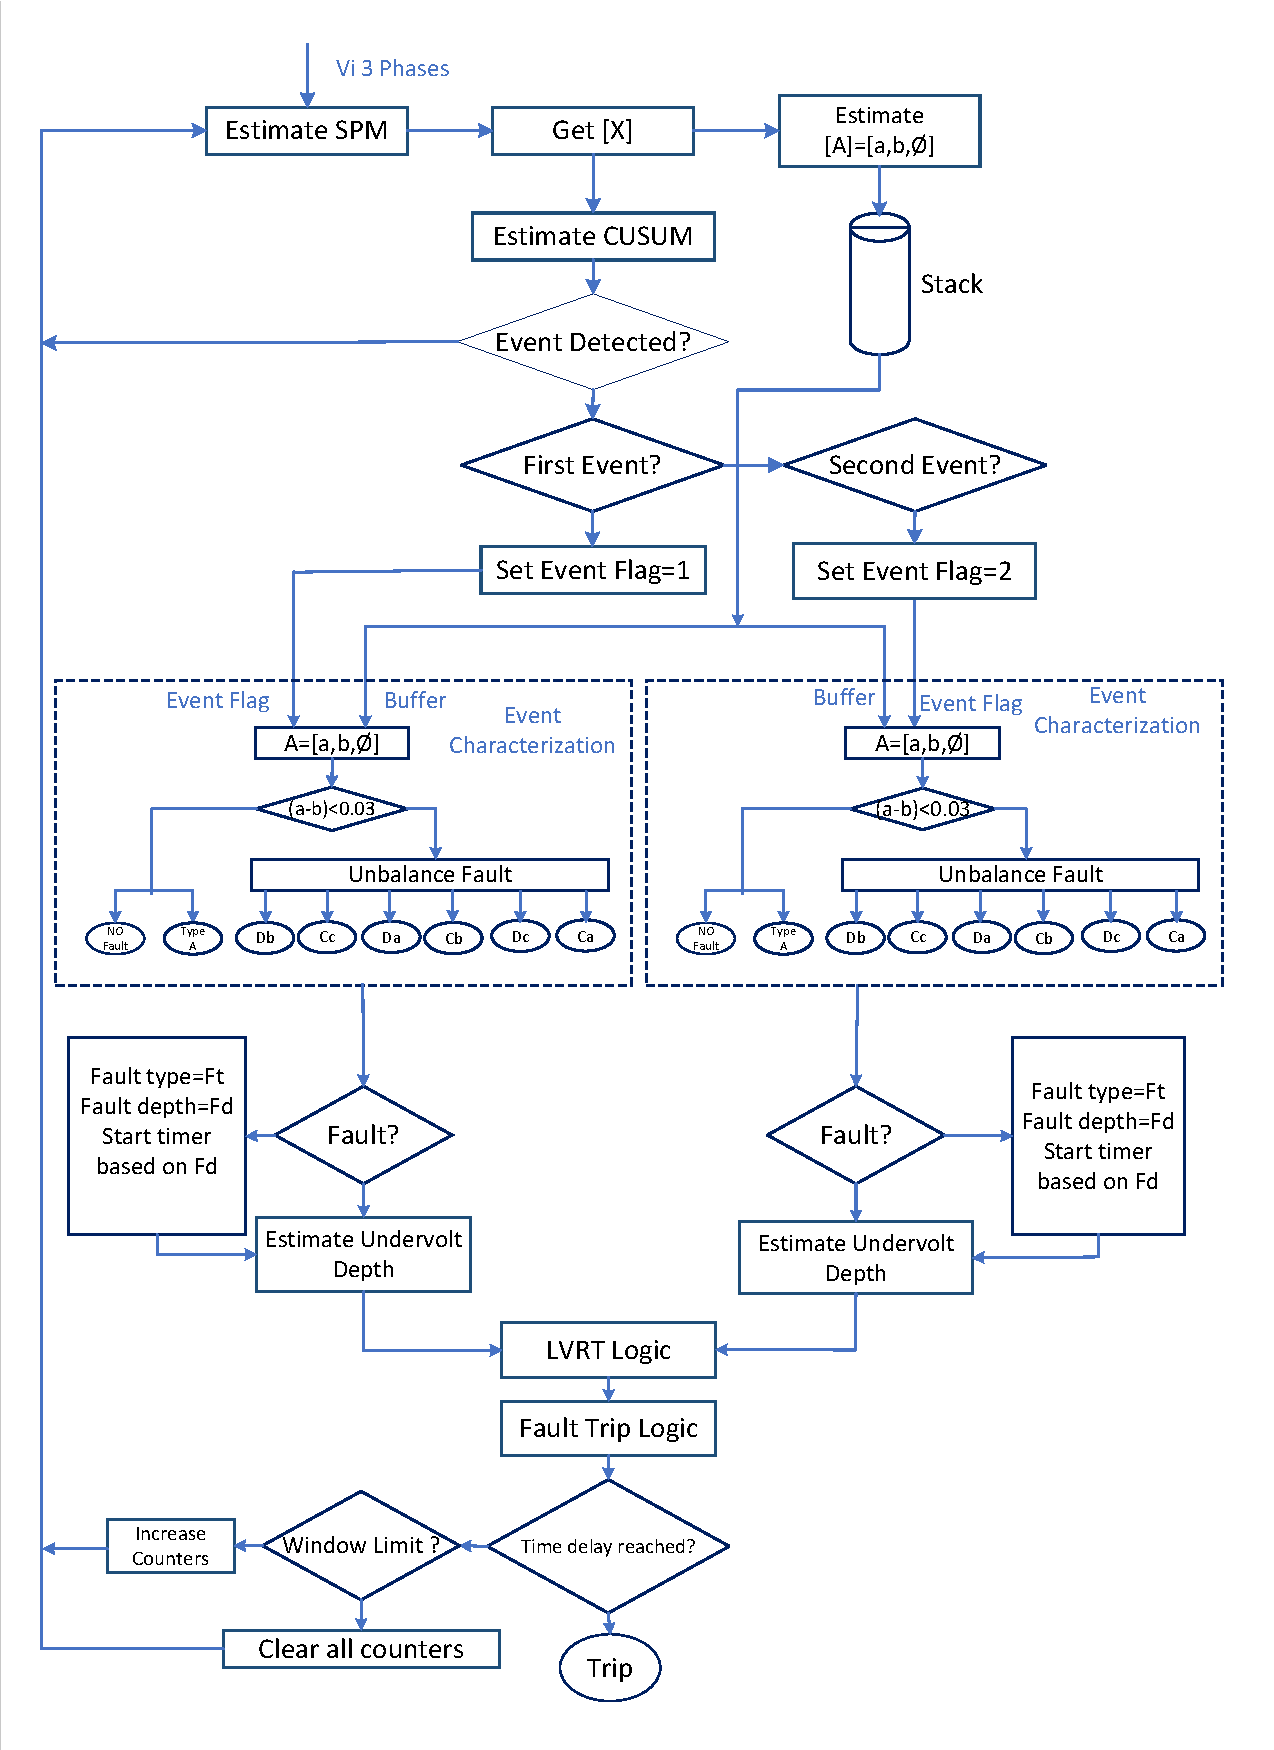
\includegraphics[page=1,  scale=0.6, trim={10 10 10 10}, clip]{images/chapter_3/eluva6.pdf}
\caption{Algorithm for proposed Enhanced Voltage Protection Module (EVPM)}
\label{flowchartref}
\end{figure*}



\begin{table}[!h]
        \caption{Shall-trip voltage default settings for Category III DER based on IEEE 1547-2018 standard~\cite{IEEE1547}}.
	\label{LowvolttriptimesIEEE}
    \centering
    \begin{tabular}{|c|c|c|}
    \hline
        Shall trip  
 & Default settings  & Default settings \\ \hline
        function & Voltage  (p.u) & Clearing time (s)  \\ \hline
        OV2  & 1.2 & 0.16 \\ \hline
        OV1  & 1.1 & 13 \\ \hline
        UV1  & 0.88 & 21 \\ \hline
        UV2 & 0.5 & 2 \\ \hline
    \end{tabular}
\end{table}


\subsection{EVPM algorithm}
A flowchart illustrating the EVPM algorithm is shown in Figure~\ref {flowchartref}.~It has four stages.~Initially, feature extraction was performed, which included the following estimations.~The three-phase to neutral voltages monitored at the IPR terminals were processed to obtain the fundamental frequency components.~Subsequently, the SPM for these voltage measurements is computed, yielding an SPM vector [X] as represented in (11), which is stored. ~Subsequently, the ellipse parameters are estimated from the SPM vector using a moving window of one cycle duration consisting of 68 samples. The method of least-squares, as discussed in the previous section, was employed to determine the major axis ($a_\text{i}$) length, minor axis ($b_\text{i}$) length, and angle of tilt ($\phi_\text{i}$) of the ellipse.~These calculated values are saved as an array to form the characteristic vector A =[$a_\text{i}$, $b_\text{i}$, $\phi_\text{i}$].~The voltage sag is characterized based on the estimated parameters of the SPM plot until another event is triggered, thereby predicting the underlying cause of the voltage sag.

Event detection is performed in the second stage.~An event is triggered for an under-voltage less than 0.85 PU or an over-voltage event greater than 1.05 PU. Under normal operating conditions, characteristic matrix A maintains a constant value of~[$a_\text{i}$,~$b_\text{i}$,~$\phi_\text{i}$]~=~[1,1,0] which changes following a fault event. Variations in the minor axis length (CV) are assessed to trigger the event flag by employing the two-sided cumulative sum (CUSUM) algorithm to calculate this change\cite{basseville1993detection}.~Once the event flag is set, event characterization is ensured in the subsequent step, accompanied by the initiation of a delay counter to estimate the time elapsed after event detection.

In the third stage of the algorithm, event classification occurs, which involve the classification of fault severity and types based on ellipse parameters.~The mean values of $a_\text{i}$, $b_\text{i}$, and $\phi_\text{i}$ were analyzed for each event to characterize the voltage sag.~A difference index, calculated as the absolute difference ($ \mid a_\text{mean}$ - $b_\text{mean} \mid $), aids in distinguishing between unbalanced and balanced dips.~In addition, unbalanced faults are further categorized into various types based on the tilt angle of ellipse $\phi_\text{i}$.~This event characterization, relying on estimated ellipse parameters, utilizes a decision tree to classify voltage sag types (shown in Figure~\ref {flowchartref}) which categorizes voltage sags into A, C, and D types.~Following the fault detection in the event detection and characterization stages, the fault flag was set to 1. At this point, the EVPM is unable to determine the fault zone because a voltage sag can affect a large part of the network.~The EVPM must synchronize with the overcurrent relays in the host distribution system. Once the fault flag is set, the EVPM awaits the next event before tripping the DG during the decision-making stage. The duration for which EVPM waits before tripping the DG depends on the operating time of the overcurrent relay in the host network. If the faulty section of the distribution system is isolated, EVPM in healthy sections observes that CV and PNF return to nominal values above the thresholds, thus preventing tripping.

In the fourth stage of the algorithm, decision-making is performed. A second voltage sag event was detected upon opening the upstream relay. The fault flag is set for the first event, whereas the event flag for the second event indicates the opening of the recloser. If the PV DG sources inject current, the fault characteristics remain unchanged. The fault type persisted even after the recloser opening, ensuring the existence of faults and tripping conditions for the EVPM. The trip signal is initiated at time $t_1$. The time coordination chart in Figure~\ref{relaytriptimes} shows the operational timing of EVPM in sync with the upstream relay, source LVRT, and islanding detection time. If the upstream relay fails to operate, the PV DG unit is isolated from the host distribution feeder at time $t_2$. If a downstream relay clears the fault, the CV and PNF return to nominal values above the thresholds, and a block signal is issued to prevent IPR tripping.

The undervoltage protection setting characterization chart for the EVPM, as depicted in Figure~\ref{flowchartref}, illustrates the locus for the Cc fault type. The complex plane was partitioned into sectors of 30°, and the fault types were derived based on the estimated tilt angle. The depth of the voltage sag was determined using the CV magnitude. Two distinct delay settings were defined at 0.88 PU and 0.5 PU. 
The numerical values of the CV and PNF corresponding to these settings are listed in Table~\ref{flowchartref}.~The various fault types are described in column 1.~The voltage magnitudes of three phases for various fault types for a voltage dip of 0.5 PU are shown in column 2 through Column 4.~The derived values of CV and PNF corresponding to each fault type are shown in columns 5 and 6, respectively.~Similarly, voltage magnitudes of three phases for different fault types for a voltage dip of 0.88 PU are given in column 7 through column 9.~The corresponding CV and PNF values are given Columns 10 and 11 respectively.~The  derived tilt angles are listed in Column~12.

\section{Adaptive recloser coordination}
Traditional auto-reclosing schemes (ANSI 79) operate on fixed time intervals, assuming a radial system where the utility can safely re-energize the line once the transient fault (e.g., a lightning strike) clears. In the presence of distributed generation (DG), however, fixed reclosing poses a severe risk of out-of-phase reclosing, which can mechanically damage DG units or cause system-wide instability.

Adaptive Reclosing utilizes real-time monitoring to confirm that:
\begin{itemize}
    \item The fault is indeed transient and has been fully extinguished.
    \item The islanded portion of the grid has either been fully disconnected or is precisely synchronized with the utility voltage and frequency before the breaker closes.
    \item The system response distinguishes between active faults involving current flow and passive faults that alter parameters without direct short circuits.
\end{itemize}




\section{Advanced Islanding Detection}
Utilizing $Q$-sign and $V$-magnitude to resolve directional ambiguity during IBR reactive current injection.

Standard directional elements (ANSI 67) rely on the phase relationship between the operating current and a polarizing voltage. However, the control loops of IBRs—specifically during Low-Voltage Ride-Through (LVRT)—often inject a high percentage of reactive power ($I_q$) to support the grid voltage. This injection can cause the fault current to lag the voltage by nearly $90^\circ$, potentially falling into the "non-trip" region of a standard directional relay.
Enhanced schemes utilize:
\begin{itemize}
    \item \textbf{Reactive Power ($\mathbf{Q}$) Sign:} Monitoring the direction of reactive power flow to determine fault location relative to the Point of Interconnection (POI).
    \item \textbf{Voltage-Phase-Angle ($\mathbf{\Delta \theta}$) Jump:} Identifying faults based on the sudden shift in voltage phase angle, which is often more reliable than the suppressed current signatures of current-limited inverters.
    \item \textbf{Symmetry Analysis:} Differentiating between symmetrical (3-phase) and unsymmetrical (L-G, L-L) faults based on the resulting phase imbalance.
    \end{itemize}

% \subsection{Negative Sequence Overcurrent (ANSI 46)}
Enhancing sensitivity to unbalanced faults (L-G, L-L) that are often suppressed by inverter controllers.
% \subsection{High Impedance Fault (HIF) Detection}
Utilizing the DIHZPTOC element for arcing signature identification via 3rd/5th harmonic analysis.

\begin{figure}[!ht]
\centering{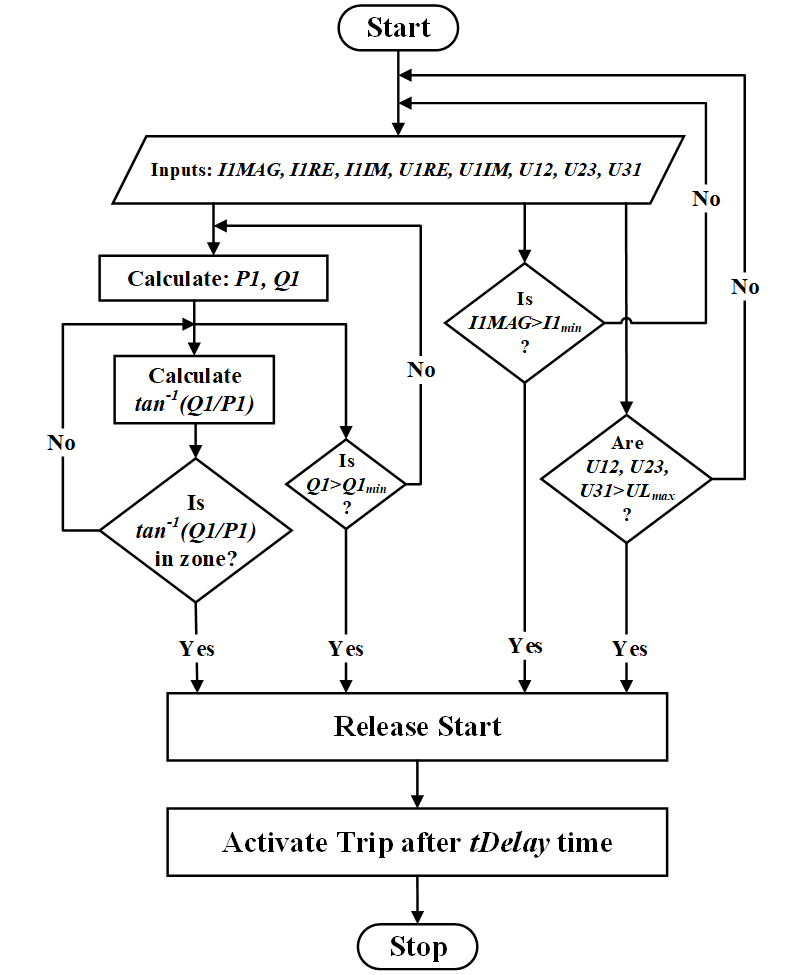
\includegraphics[width=0.75\textwidth]{images/chapter_3/Drawing1.png}}
\caption{Algorithm for advanced islanding detection.\label{Fig2}}
\end{figure}
%%%%%%%%%%%%%%%%%%%%%%%%%%%%%%%%%%%%%%%%%%%%%%%%%%
\section{Performance evaluation of fault phase selection logic, EVPM and adaptive reclosing}

The performance of the proposed fault phase selection logic, EVPM and adaptive reclosing for IPR is assessed through transient simulation studies conducted in three case-study networks using PSCAD/EMTDC, considering various fault scenarios.




\subsubsection{Phase Selection Accuracy:}
While IBRs often suppress negative sequence currents ($I_2$), making L-G and L-L identification difficult for standard relays, the EVPM identifies the fault type based on the tilt angle ($\phi$) of the ellipse.

\subsubsection{EVPM Precision:}
The EVPM utilizes the Space Phasor Model (SPM) to transform circular healthy states into elliptical fault states, providing a clear "signature" for various fault types.\\
 Validation against Industrial Benchmarks: Testing the EVPM against standardized voltage dip profiles.\\
 Speed and Selectivity Analysis: Demonstrating the 12 ms classification speed of the EVPM versus the 40 ms standard in traditional RMS relays.\\
 Case Study Synthesis: Comprehensive validation across PPU 11 kV, CIGRE MV Benchmark, and Multi-DG microgrids.\\
\subsubsection{Sensitivity to Fault Signatures in Inverter-Based Resources (IBRs)}
In the CIGRE benchmark, which integrates Type 4 wind farms and PV plants, traditional protection coordination degrades due to bidirectional flows and current-limited signatures.
\subsubsection{RMS Limitations:}
Conventional undervoltage functions (ANSI 27) rely on the root mean square of voltages, making it difficult to differentiate between faults and non-fault events like motor starting or transformer saturation.
\subsubsection{Coordination with Host-Network Reclosers}
A primary objective of the EVPM is to synchronize with upstream line reclosers (ANSI 79) to ensure the isolation of DGs before a reclosing attempt occurs.
\subsubsection{Conventional Delay:}
In common practice, reclosing attempts must be delayed (often from 0.3s to 1s) to ensure DGs are isolated, leading to increased power interruption times.
\subsubsection{EVPM Acceleration:}
The EVPM senses the inception of a fault and the subsequent first operation of a recloser as a multi-stage voltage dip.
\subsubsection{Instantaneous Decision:}
By detecting that the fault persists after the recloser opens ($t_{r1}$), the EVPM issues a trip command ($t_{Ip1}$) without the extensive time delays required by RMS-based functions.

\section{Comparative Case Studies}

Case study 1:~A single PV source integrated into an 11~kV distribution feeder through an IPR, as depicted in Figure~\ref{flowchartref}, is considered for case study 1.~A comprehensive study of various fault types, including balanced and unbalanced faults at different locations on the feeder and with varying fault impedances, are conducted.~The various study cases are summarized in Table~\ref{flowchartref}.~The detailed waveform analysis for selected cases are presented in the subsequent sections.

Case study 2:~A single-feeder distribution network, adapted from the CIGRE benchmark system for network integration studies (Figure~\ref{cigreevpm}), is considered for case study 2.~This is a representative of European MV distribution network based on an actual physical system.~Multiple PV sources are integrated into the network via IPRs.~Table~\ref{flowchartref} outlines the diverse fault scenarios considered, including different fault types at various locations on the feeder and with varying fault impedances.~The estimation of SPM parameters by the EVPM using measured three-phase voltages for selected fault events are detailed in the subsequent sections.

Case study 3: A 20 kV distribution test feeder (Figure~\ref{flowchartref}), integrated with diverse distributed energy sources including a DFIG wind farm, a PV system, a PV-battery system, and a diesel generator, is considered for case study~3. ~The analysis also includes a variety of ZIP load types. ~Table~\ref{flowchartref} summarizes the different fault cases analyzed, encompassing a range of fault locations and fault impedances on the feeder. ~The following sections present the SPM parameters estimated by the EVPM using measured voltages during selected fault events.

\subsection{Case study 1: Evaluation of EVPM Performance in a~11~kV distribution feeder integrated with a single PV source}
The utility source is modeled as a constant voltage source with a short-circuit capacity of 120 MVA at the substation bus.~The line parameters are listed in Table \ref{flowchartref}.~The nominal voltage rating of the primary distribution feeder is 11~kV.~ A reclosing relay (79) is installed at the beginning of the feeder to provide overcurrent protection.~The PV source is connected to the feeder through an interfacing transformer.~The IPR is connected to the PCC.~The PV source has a maximum capacity of 4~MW and operates at a nominal voltage of 4.6~kV.~The inverter is modeled as a full-scale voltage source converter (VSC), which functions in constant power control mode.~The VSC controller is implemented in a rotating reference frame with an independent real and reactive power control~\cite{teodorescu2011grid}.~LVRT control is implemented for the PV source, and the settings suggested by the Central Electricity Authority (CEA) of India are taken as an example~(Figure~\ref {flowchartref})\cite{cea}.~The maximum fault current capacity of the PV source is limited to 1.5 PU by a limiter in the control loop.~The converter is designed to operate with a unity power factor during a fault in the distribution feeder.~The interfacing transformer is 5~MVA, rated at 4.6/11~kV with a DyG configuration and an impedance of X = 0.07~PU.~Subsequent studies evaluate the tripping time of conventional RMS-based undervoltage functions (27) used in multi-function IPR when LVRT has adhered to faults in the host network against the time required to isolate the fault when EVPM is implemented.~A detailed analysis is provided below.~Table \ref{flowchartref} lists the fault cases analyzed, encompassing a variety of fault types, locations, and impedances on the feeder.~A comprehensive waveform analysis of selected cases is discussed in the following section.




\begin{figure}[t!]
	\centering
	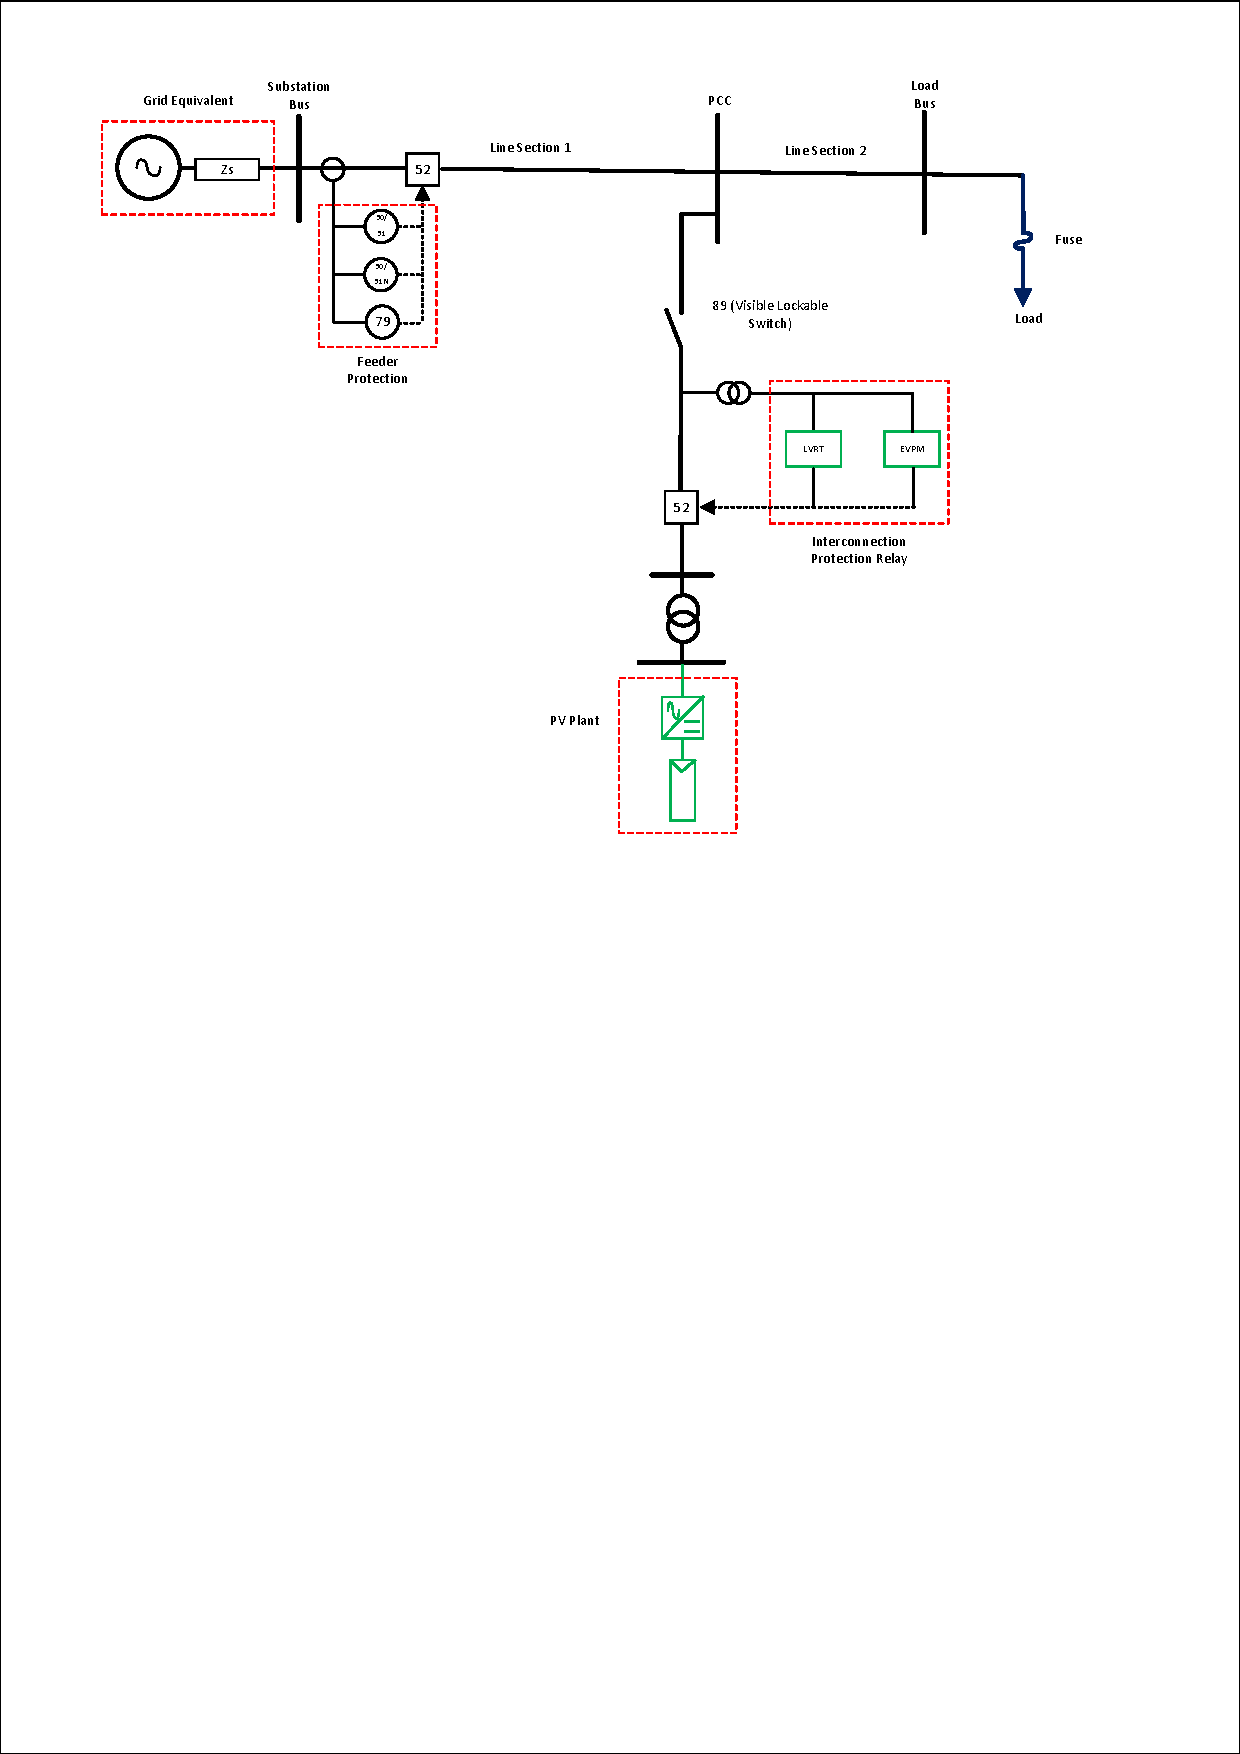
\includegraphics[page=1, scale=0.55, trim={20 420 20 30}, clip]{images/chapter_3/eluva8.pdf}
	\caption{Study case network, a single PV source connected to an 11kV distribution feeder via IPR.}
	\label{Fig23}
\end{figure}


\begin{figure}[h!]
	\centering
	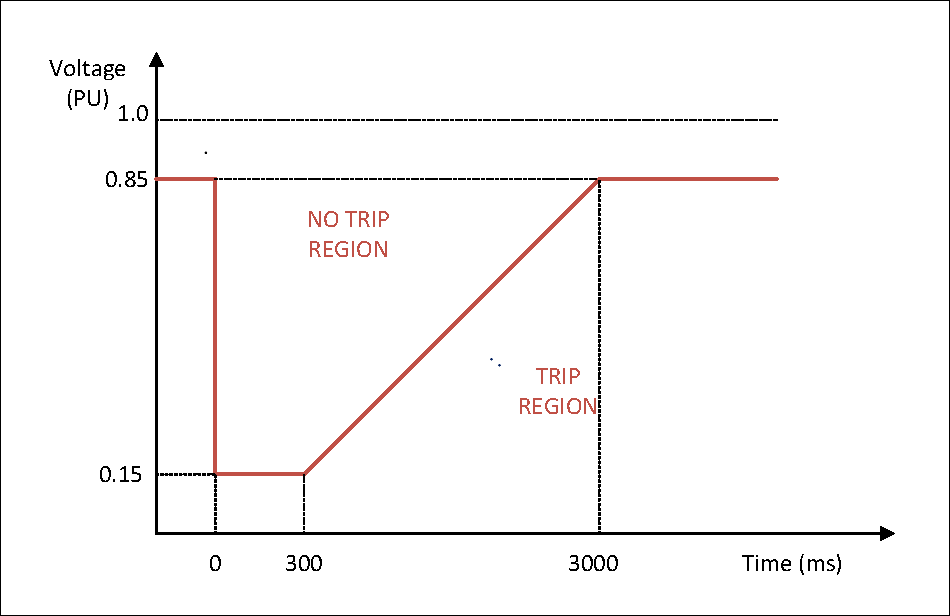
\includegraphics[scale=0.55, trim={20 20 20 25}, clip]{images/chapter_3/LVRT_India.pdf}
	\caption{LVRT requirements according to Indian standards~\cite{cea}.}
	\label{Fig24}
\end{figure}





\begin{figure}[!ht]
\centering{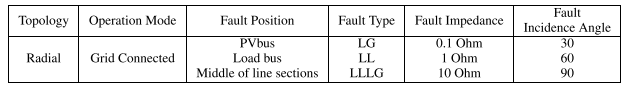
\includegraphics[width=0.75\textwidth]{images/chapter_3/SimulationCircuit1a.png}}
\caption{Study case network, a single PV source connected to an 11kV distribution feeder via IPR.
\label{Fig25}}
\end{figure}



%%%%%%%%%%%%%%%%%%%%%%%%%%%%%%%%%%%%%%%%%%%%%%%%%%%%%%%
\subsubsection{Single phase to ground fault}
A single line-to-ground fault (phase B to ground) is simulated on the primary distribution feeder at the load bus during a simulation time of t = 2 seconds. In the first scenario, the time taken for the IPR to trip when  LVRT is followed is analyzed. The three-phase to neutral voltages measured at the IPR terminals are illustrated in Figure \ref{Fig23} (a). The RMS values of the voltages for all three phases were estimated using a single-cycle Discrete Fourier Transform (DFT), as shown in Figure \ref{slglvrtthreephase} (b). The LVRT controller calculates the trip time based on the voltage dip value of the lowest of the three voltages.~Figure~\ref{Fig24} displays the estimation of the tripping time using the RMS voltage on the LVRT curve. It can be observed from Figure \ref{lvrtslg} that after the fault event, the voltage crosses the threshold of 0.85~pu, and the counter is initiated. At this point, the voltage is in the no-trip region. The second voltage dip occurs after the recloser opens, 0.15 seconds after the fault. The estimated time for the voltage to enter the trip region in the LVRT curve is 0.55 seconds. Consequently, the trip signal from the IPR is given 0.55 seconds after the fault's onset, and the PV DG trips at 2.55 seconds, as shown in Figure~\ref{Fig25}.

In the following scenario, the trip time estimated by EVPM using the algorithm discussed in Section~(IV) is analyzed.~EVPM estimated the SPM for the measured three-phase voltages and its projection on the complex plane, as shown in Figure~\ref{polarslg}.~The shape of the SPM changed from a circle to an ellipse because of the fault event.~The SPM is divided into segments of multiple events, as shown in Figure~\ref{Fig23}.Variations in the estimated ellipse parameters are shown in Figure \ref{Fig23}~(b). ~A change in the CV was detected that triggered the event flag.~The fault type is estimated using the calculated tilt angle of the ellipse.~The angle of inclination changes from $0^o$ to $ 26.52^o$ (0.462 rad), and the dip type is estimated as $D_b$.~The variation in the tilt angle of the ellipse is shown in Figure~\ref{Fig23}~(c).~The EVPM counter starts as the CV crosses the threshold and the fault flag is set.~The upstream recloser opens in a time duration of 2.15 s and the second voltage dip due to recloser opening is sensed at the IPR terminals.~After the recloser opening, the CV values have the second change at which event flag sets.~The fault flag was set for the first event, and the event flag for the second event indicated a recloser opening.~The estimated tilt angle is $ 29.54^o $(0.515 rad), corresponding to fault type $D_b$.~The dip type remains the same after the recloser opening, ensuring the existence of a fault and the persistent tripping condition for the EVPM.~A trip command was given with an intentional delay of 0.1~s.

%%%%%%%%%%%%%%%%%%%%%%%%%%%%%%%%%%%%%%%%%%%%%%%%%%%%
% \begin{figure}[!ht]
% \centering{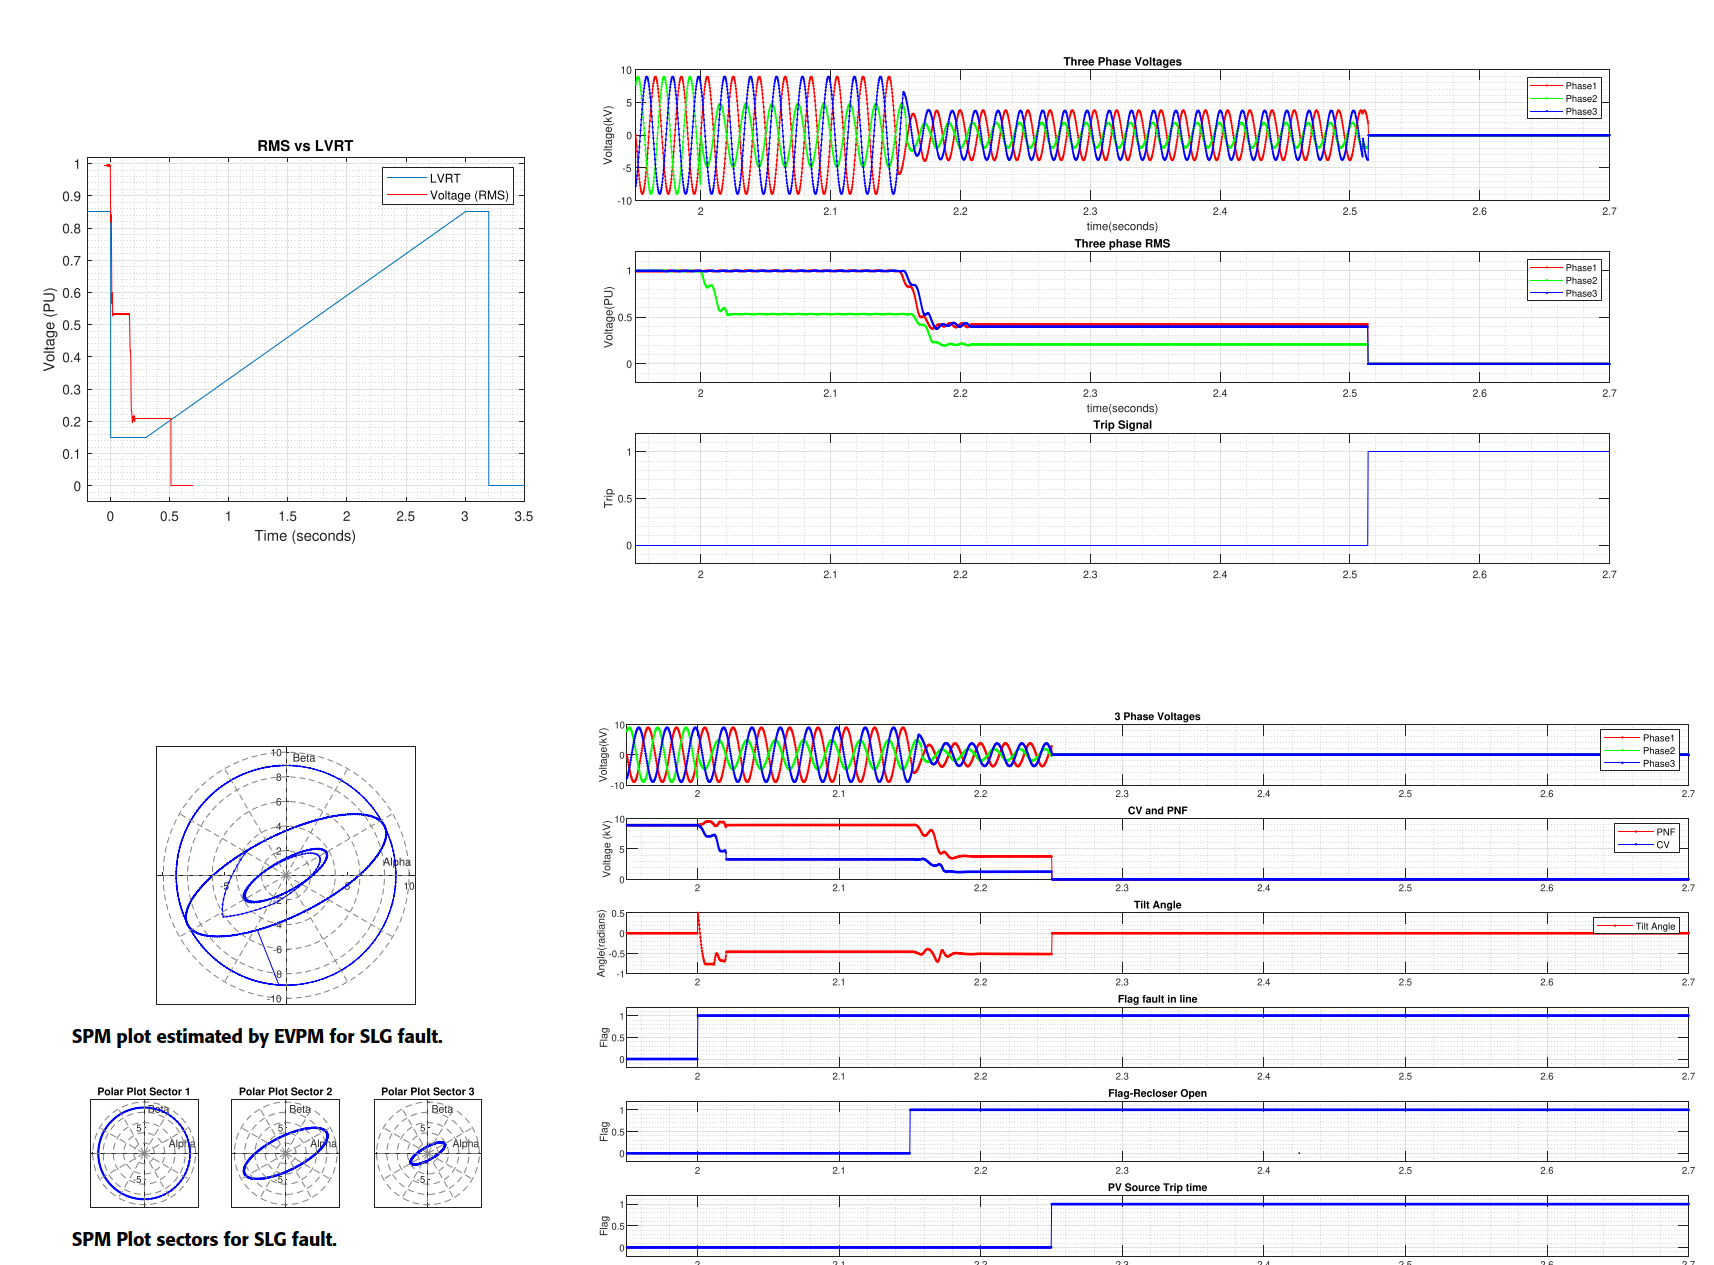
\includegraphics[width=0.75\textwidth]{images/chapter_3/SimulationCircuit1Result1.png}}
% \caption{Various Case Studies.\label{Fig2}}
% \end{figure}\


\begin{figure}[h!]
    \centering
\begin{minipage}{0.8\textwidth}
        \centering
        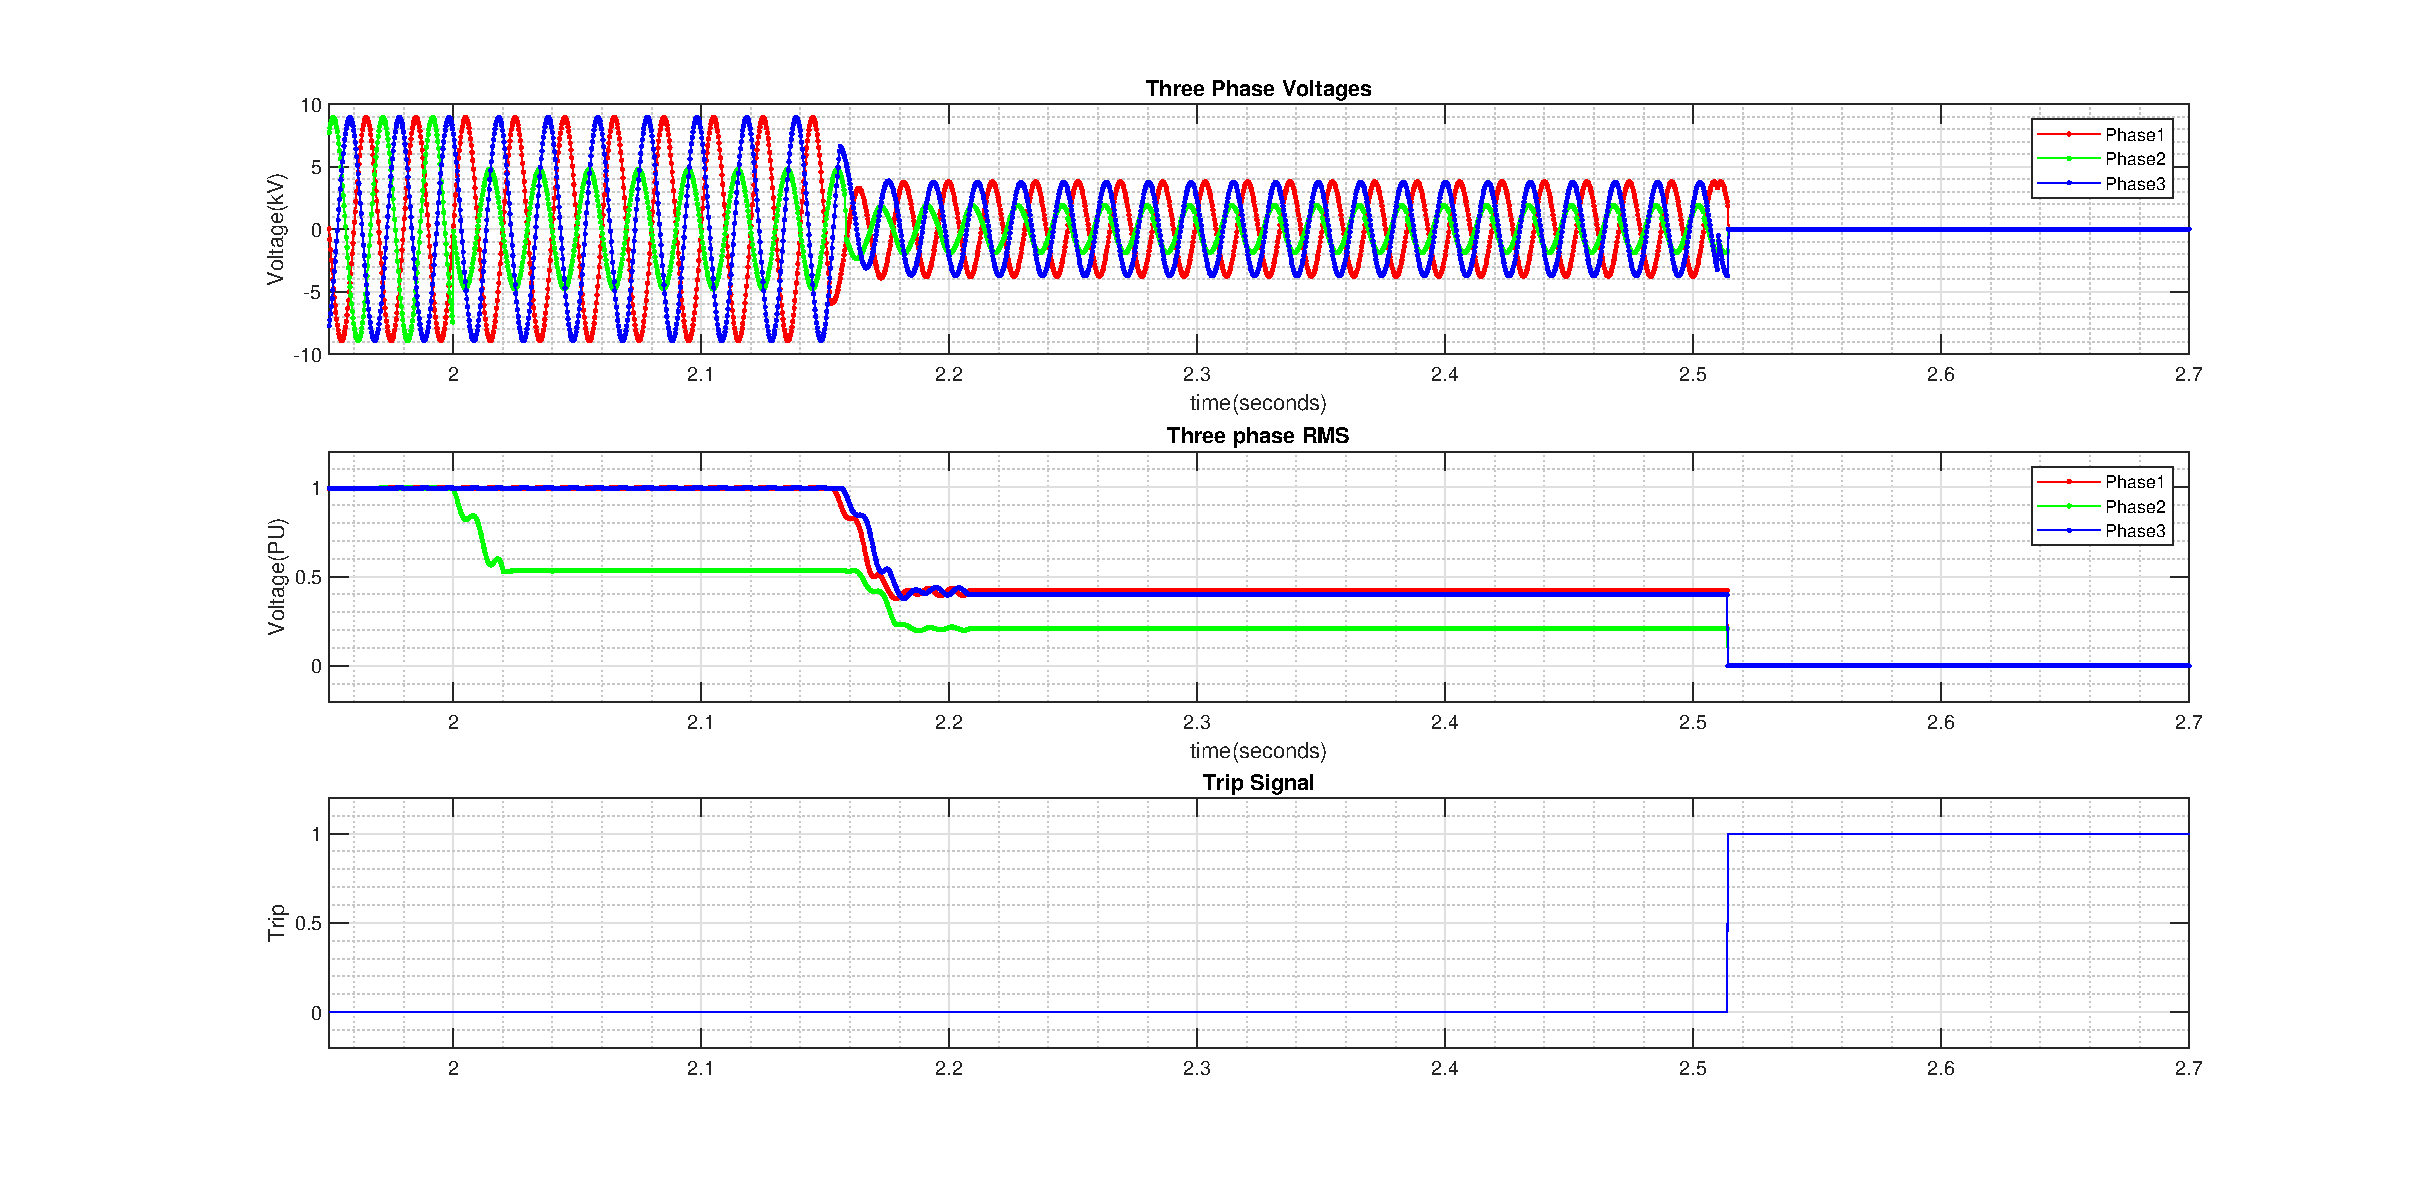
\includegraphics[width=0.9\textwidth, trim={50 10 50 30},clip]{images/chapter_3/20threephaseRMStripSLG.eps}% Big image
        \vspace{-0.5cm}
        \caption{Trip time of conventional RMS-based undervoltage functions (27) used in multi-function IPR when following LVRT, for a SLG fault.}
	\label{slglvrtthreephase}
  
    \end{minipage}\hfill
    \vspace{0.25cm}
    \begin{minipage}{0.5\textwidth}
        \centering
        %\includegraphics[width=\textwidth]{image1.jpg}
        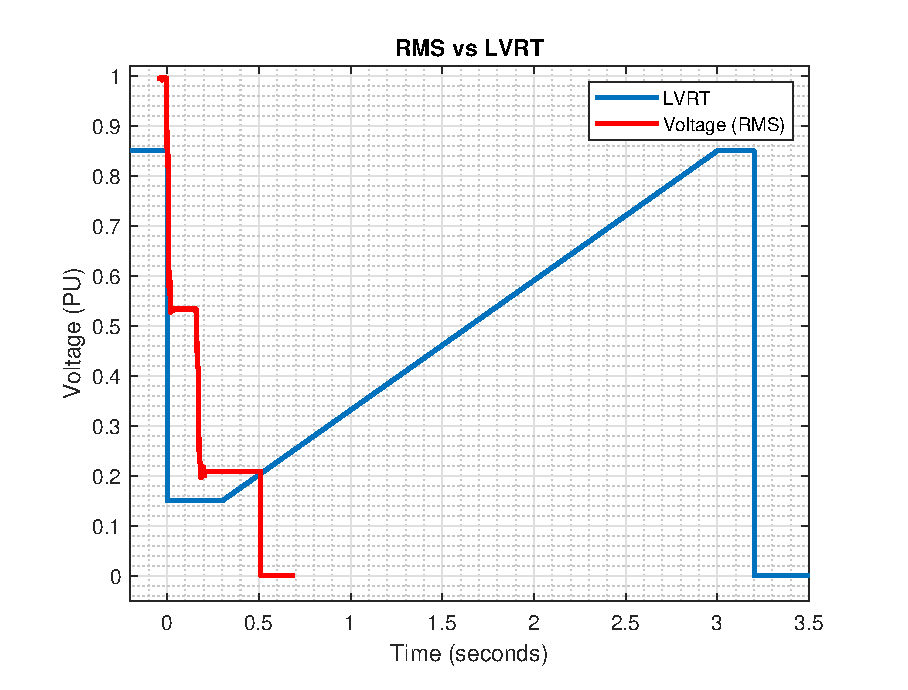
\includegraphics[width=0.8\textwidth, trim={10 2 10 10}, clip]{images/chapter_3/20LVRTonRMSNewSLG.eps}
         \vspace{-0.25cm}
        \caption{Trip time estimation by conventional RMS-based undervoltage functions (27) following LVRT.}
	\label{lvrtslg}
    \end{minipage}
    %\hfill
    \hspace{-0.1cm}
    \begin{minipage}{0.45\textwidth}
        \centering
        %\includegraphics[width=\textwidth]{image2.jpg}
        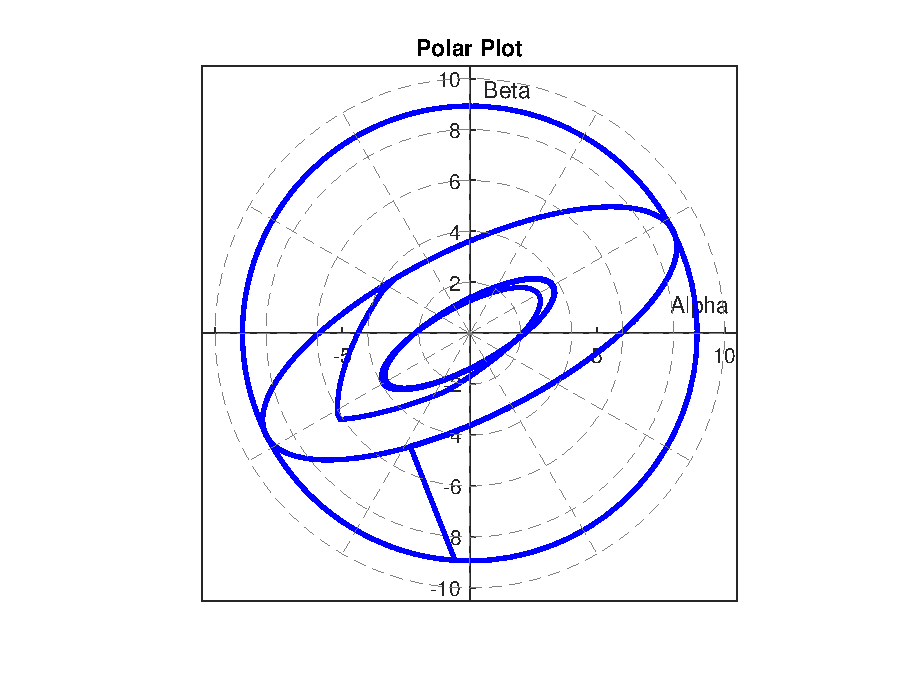
\includegraphics[ width=0.6\textwidth, trim={30 30 30 20}, clip]{images/chapter_3/20FullPlotsPolarNewSLG.eps}
        \vspace{-0.1cm}
        \caption{SPM plot estimated by EVPM for SLG fault.}
	\label{polarslg}
        \vspace{-0.1cm}
        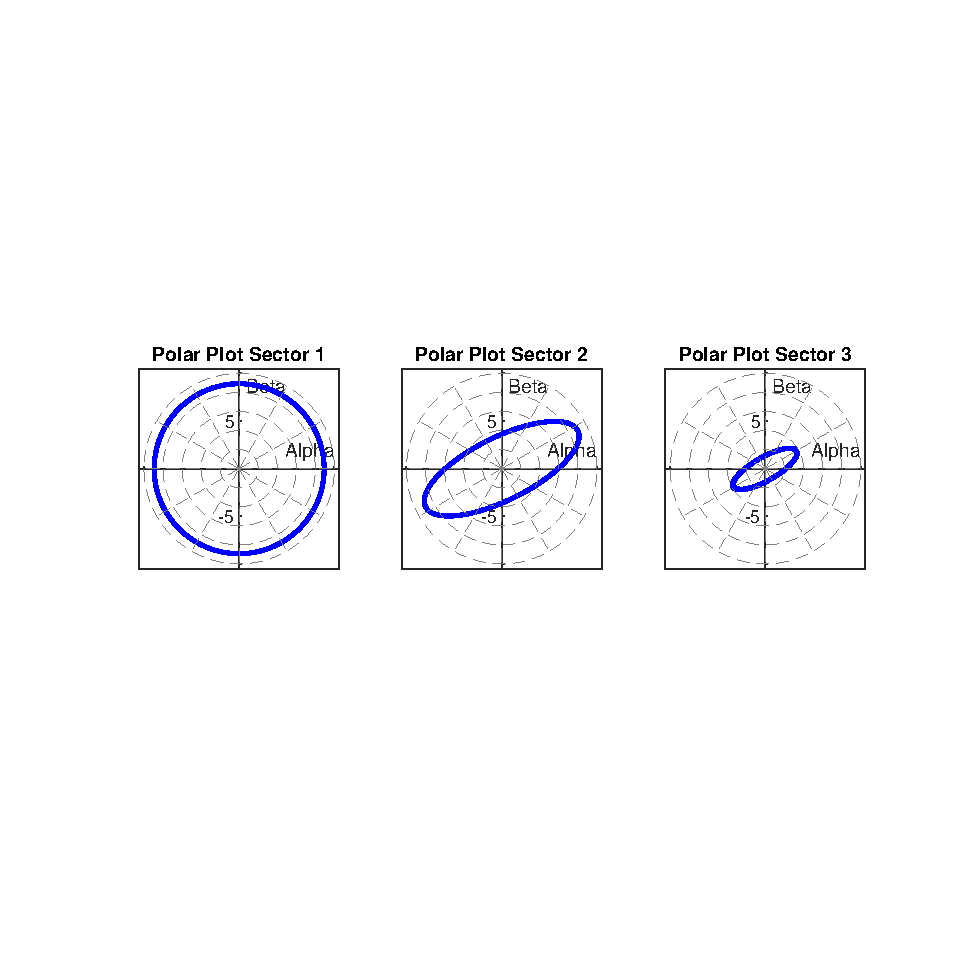
\includegraphics[width=0.8\textwidth, trim={10 180 10 150}, clip]{images/chapter_3/20PlotsPolarSectorsNewSLG.eps}
        \vspace{-0.1cm}
      \caption{SPM Plot sectors for SLG fault.}
      \label{polarslgsegments}
    \end{minipage}
\vspace{-1cm} 
  \begin{minipage}{0.8\textwidth}
        \centering
       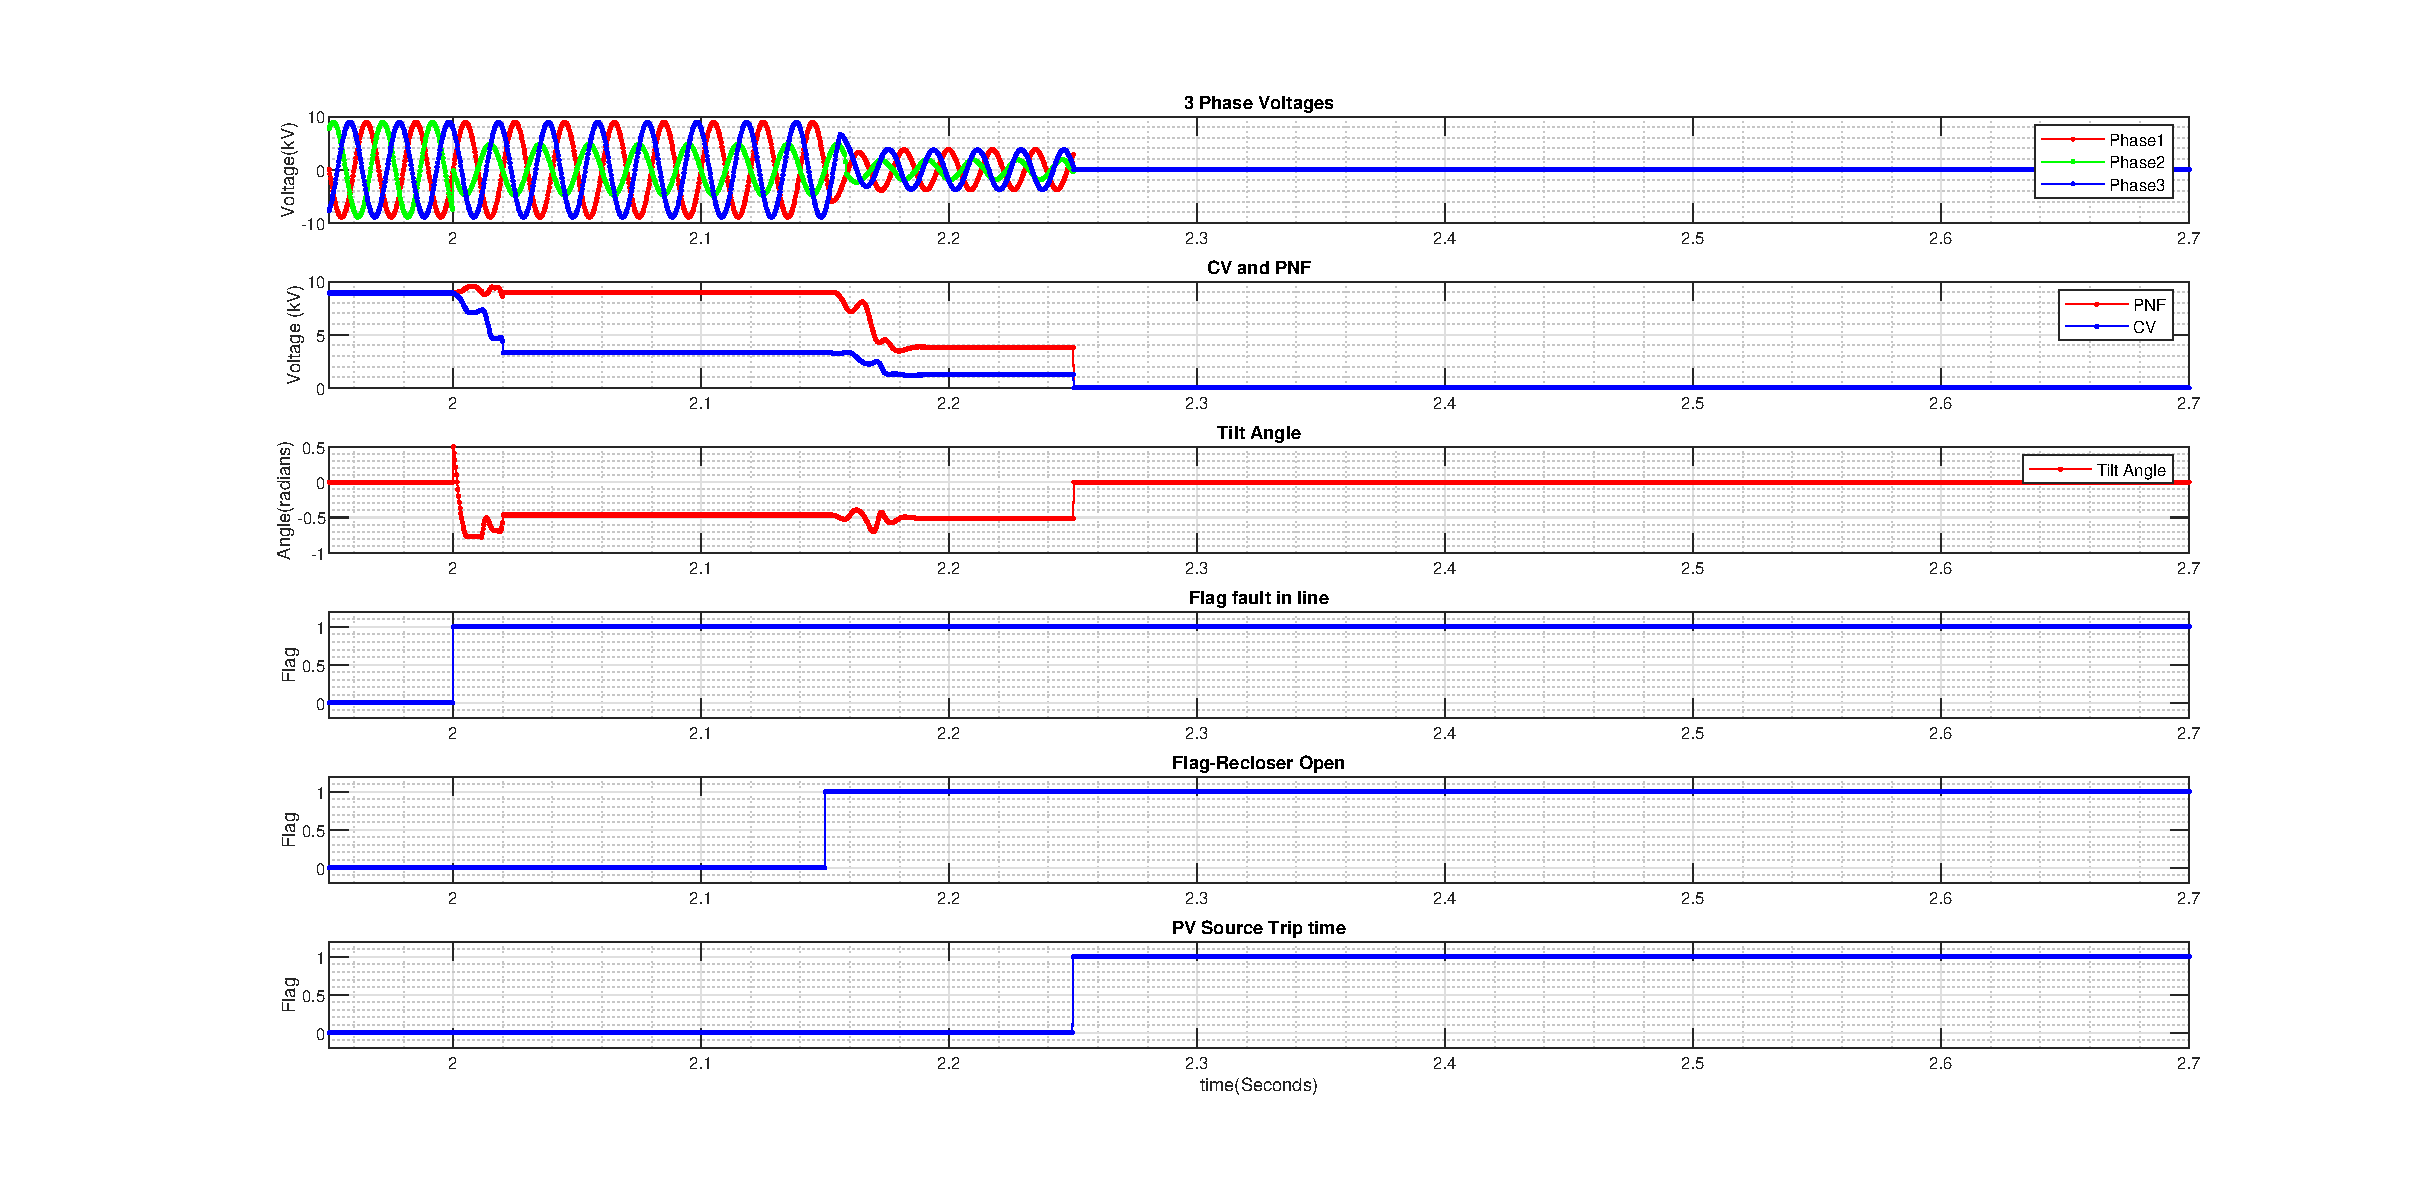
\includegraphics[page=1,width=1\textwidth, trim={70 10 10 10},clip]{images/chapter_3/20threephaseCVPNFFlagsSLG.eps}% Big image
        \vspace{-0.5cm}
       \caption{Trip time of IPR for a SLG fault when EVPM is implemented.}
	\label{slgevpm}
        \end{minipage}
\end{figure}










\begin{figure}[!ht]
\centering{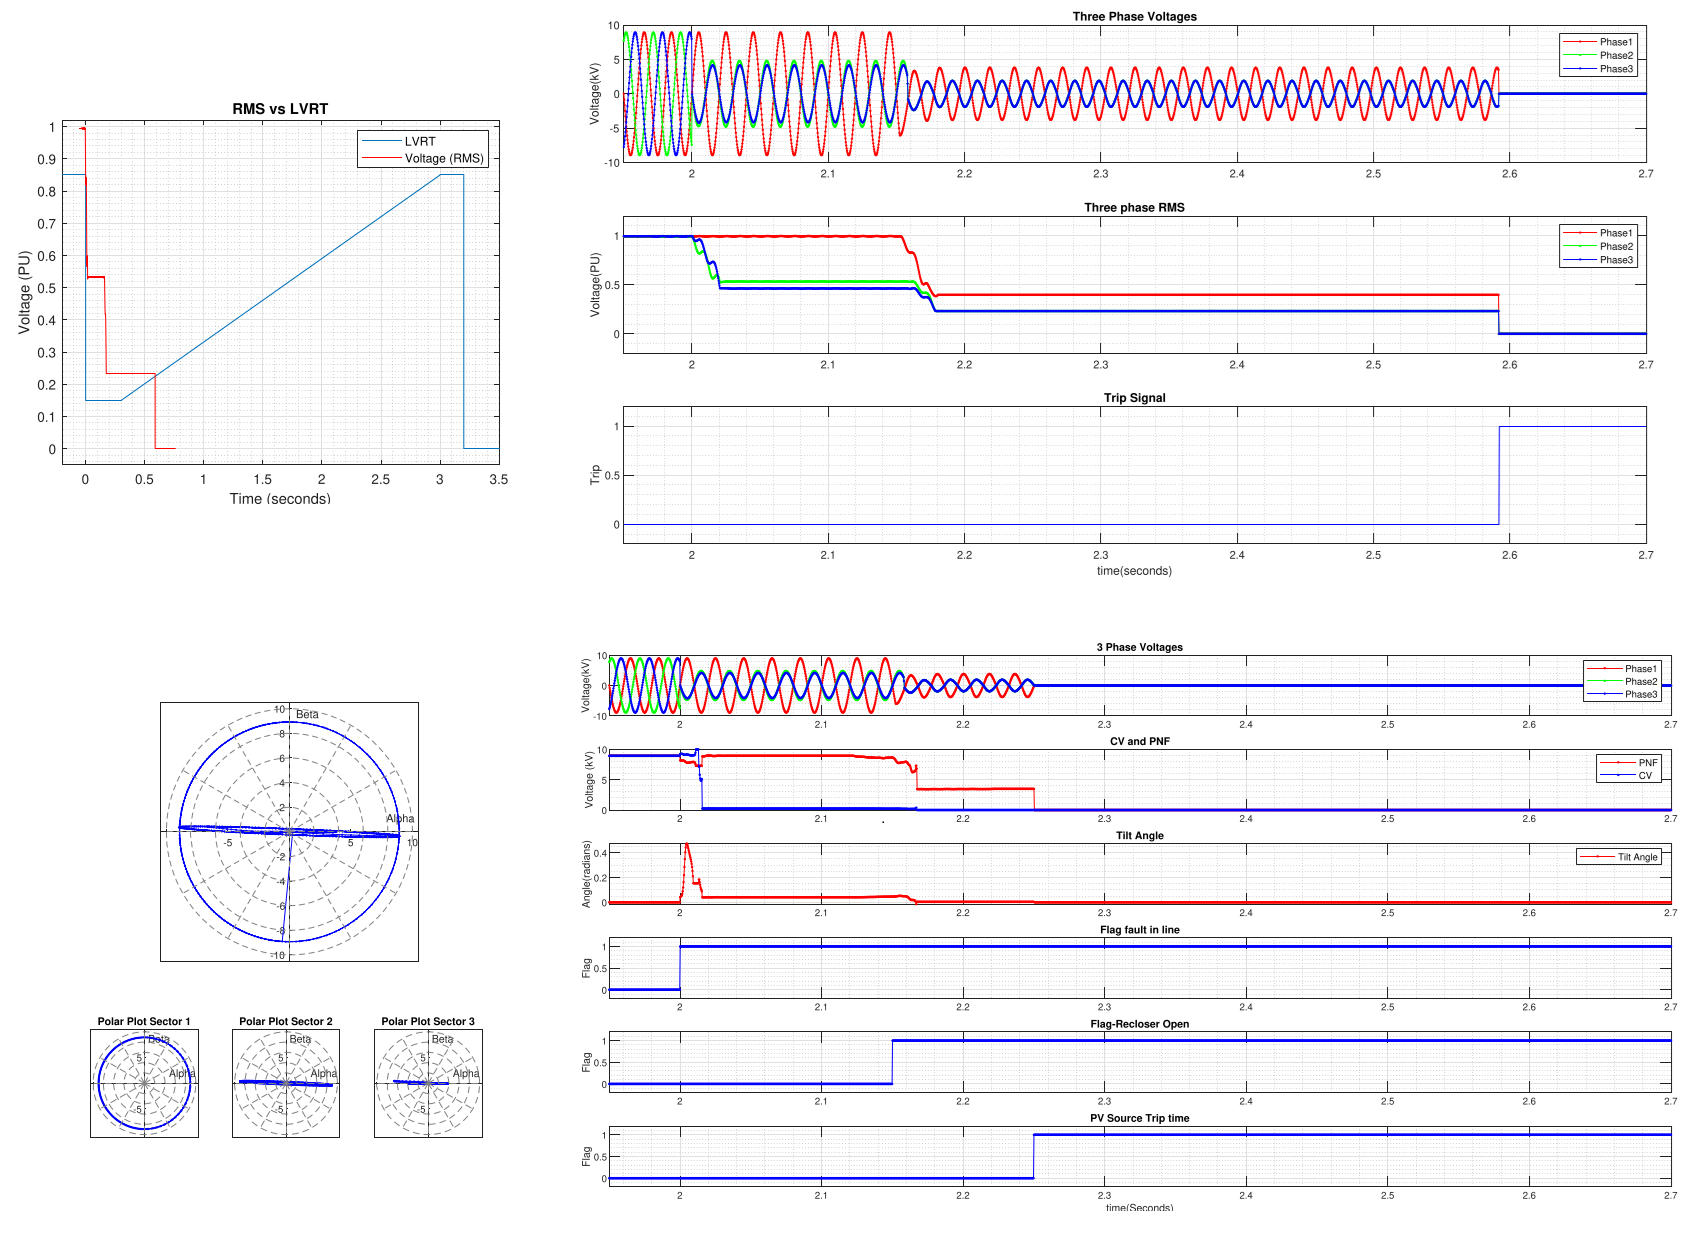
\includegraphics[width=0.75\textwidth]{images/chapter_3/SimulationCircuit1Result5.png}}
\caption{Various Case Studies.\label{Fig2}}
\end{figure}\





\subsubsection{Double line fault}


A line-to-line fault (between Phases B and C) is simulated at the load bus during the simulation at time t = 2 seconds. The three-phase to neutral voltages measured at the IPR terminals are illustrated in Figure \ref{Fig23} (a). The estimated RMS voltages for each phase are shown in Figure \ref{Fig23} (b). The LVRT controller calculates the trip time based on the voltage dip value of the lowest of the three voltages. Figure \ref{Fig23} displays the estimation of the trip time. It shows that the voltage dips below the threshold of 0.85~pu when the fault occurs. The counter begins now, indicating that the voltage is still within the no-trip region. A second dip occurs when the recloser opens. From the LVRT curve, the time estimated for the voltage to enter the trip region is 0.56 seconds. The trip signal is triggered 0.56 seconds after the fault occurs at 2.56 seconds,  as indicated in Figure \ref{Fig23}~(c). 

In the following scenario, the trip estimated by EVPM is analyzed.~The EVPM estimates the SPM for the measured three-phase voltages, and its projection on the complex plane is shown in Figure~\ref{Fig23}.~The shape of the SPM changed from a circle to an ellipse owing to the fault event.~The SPM was divided into segments of multiple events, as shown in Figure~\ref{Fig23}.~Three-phase to neutral voltages measured at the IPR terminals are shown in Figure \ref{Fig23}~(a).~The variations in CV and PNF are estimated by EVPM, as shown in Figure~\ref{Fig23}~(b).~The tilt angle is estimated to be $178^o$ (3.107 rad), indicating the fault type as $C_a$ for the first event.~The upstream recloser opens in a time duration of 0.15~s, and the voltage dip due to the recloser opening is sensed at the IPR terminals.~The dip type remained the same after the recloser opening.~A trip command is given with an intentional delay of 0.1~s.

Different fault cases were simulated, and the responses of the IPR were studied.~A summary of the EVPM measurements for the various fault types at the load bus for two different fault impedances is presented in Table~\ref{Fig23}.~The various studied fault types are listed in Column 1.~The values of CV and PNF estimated by EVPM during a fault event are given in columns 2 and 3, respectively.~ Tilt angle derived using EVPM is given in column 4.~The EVPM algorithm estimates the fault type, as shown in Column 5.~The recloser opens at 0.15 s.~After the recloser opening, a second event was triggered.~The values of CV and PNF estimated for this second event after the recloser opening are given in columns 7 and 8, respectively.~ The tilt angle estimated is given in column 9.~The fault types estimated by the EVPM algorithm are given in~Column~10.~A Comparison of the performance of conventional RMS based undervoltage relay (27) and SPM-based EVPM is given in \ref{RMSvsSPM}.

\begin{figure}[!ht]
\centering{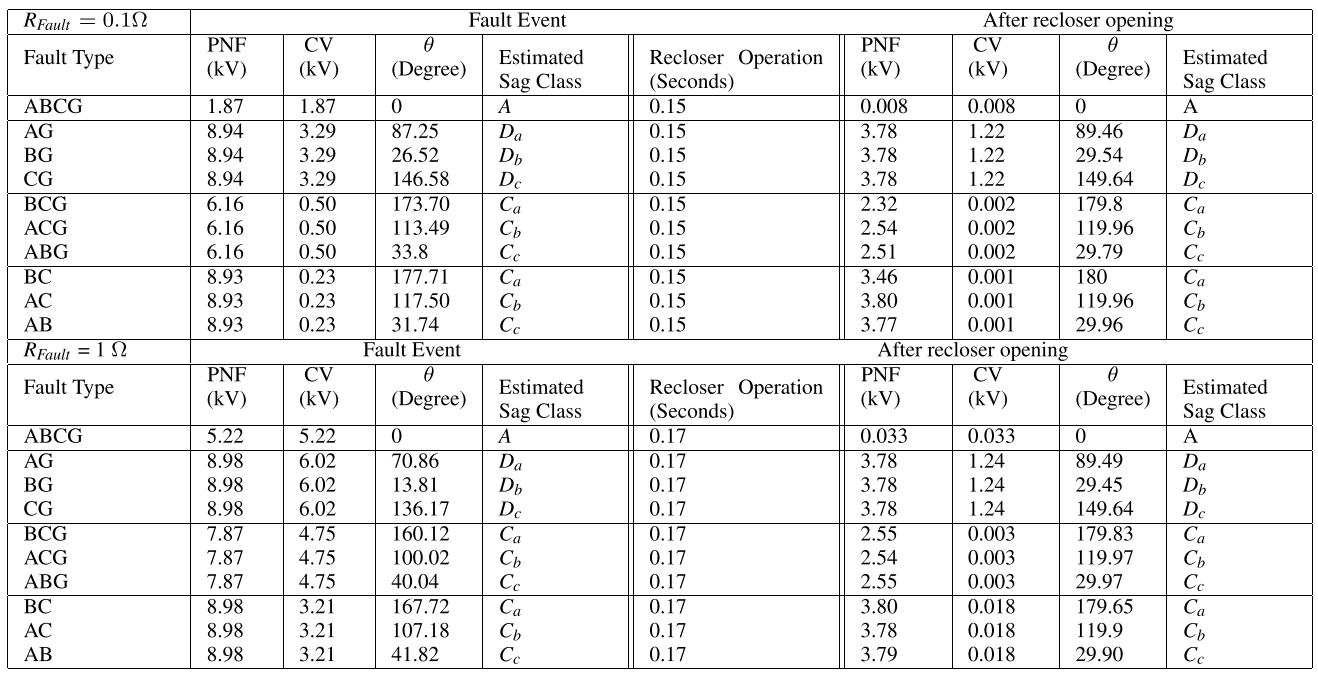
\includegraphics[width=0.75\textwidth]{images/chapter_3/FaultClassificationSimulation1.png}}
\caption{Various Case Studies.\label{Fig2}}
\end{figure}


\subsection{Case study 2: Evaluation of EVPM Performance in CIGRE European MV distribution network benchmark.}


\begin{figure}[!ht]
\centering{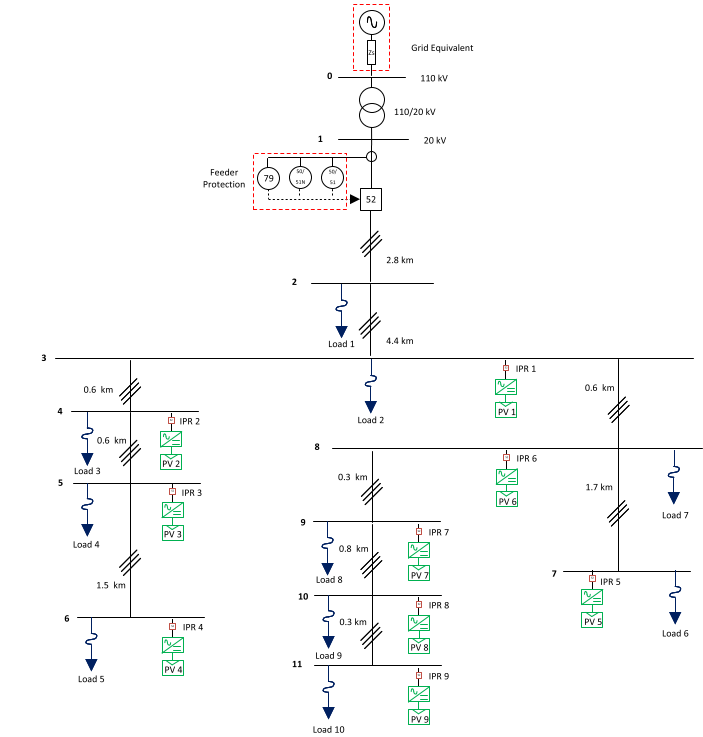
\includegraphics[width=0.75\textwidth]{images/chapter_3/SimulationCircuit2.png}}
\caption{Various Case Studies.\label{Fig2}}
\end{figure}\

\begin{figure}[!ht]
\centering{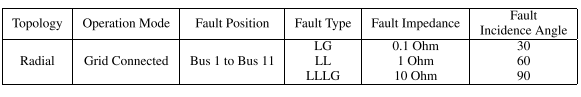
\includegraphics[width=0.75\textwidth]{images/chapter_3/SimulationCircuit2a.png}}
\caption{CIGRE benchmark system for network integration studies\label{cigreevpm}}
\end{figure}\


A single-feeder distribution network adapted from~the~CIGRE~benchmark~system for network integration of renewable and distributed energy resources studies (figure~\ref{Fig23}) is used to assess the performance of EVPM under various fault conditions \cite{cigrebenchmark}.~This network is modelled after a typical MV distribution grid in Europe.~It is based on real-world infrastructure.~The network is integrated with multiple PV DG sources connected to different buses.~The IPRs are connected at the PCC of each PV source.~The single-line diagram is depicted in figure~\ref{Fig23}.~The MV distribution feeder has a three-phase radial configuration with a nominal voltage of 20~kV and a system frequency of 50~Hz.~Unbalanced operation is not considered for this analysis, assuming a maximum unbalance of ±5\%.~The loads are fed through underground XLPE cables with round, stranded aluminium conductors and copper tape shielding.~The line parameters are given in table~\ref{Fig23}.~The distribution network supplies both residential and commercial loads with varying power factors (table~\ref{CIGRELoadDATA}).~The utility source is modelled as a constant voltage source with a short-circuit capacity of 5000~MVA at the substation bus.~The substation transformer is a three-phase Dyn1 configuration, rated at 110/20~kV and 25~MVA, with an impedance of 0.016~+~j1.92~Ohms. A recloser at the feeder's beginning provides overcurrent protection. The PV DG sources, as listed in table~\ref{Fig23}, are modelled as full-scale VSC operating in constant power control mode.~The controller utilises a rotating reference frame with independent real and reactive power control.~The maximum fault current from the PV DG is limited to 1.2~PU by a limiter in the control loop, and the converter operates at unity power factor during faults.~Table~\ref{Fig23} presents the fault cases analyzed, which include a range of fault types, locations, and fault impedances on the feeder.~The estimation of SPM parameters by the EVPM using measured three-phase voltages for selected fault events is detailed in the subsequent sections.


\subsubsection{Single phase to ground fault}

A single-phase-to-ground fault (phase A to ground) is simulated on the distribution feeder at bus 6 at a simulation time of 2 seconds. The EVPM estimates the SPM based on measured three-phase voltages and plots it on the complex plane. The fault event transforms the SPM shape from a circle to an ellipse. The parameters of the ellipse are estimated using a moving window to determine the characteristics of the single events. The SPM is segmented into sections representing multiple events, as shown in Figure~\ref{Fig23}. The fault type is estimated as a dip type based on the tilt angle of the ellipse, which changes from 0 to $88.9^\circ$. The dip type is identified as $D_a$. After the recloser opens, the values of the CV indicate a second change, which sets the event flag. The fault flag is activated for the first event, while the event flag for the second event indicates the recloser opening. The estimated tilt angle is $87.8^\circ$, which corresponds to fault type $D_a$. The dip type remains the same after the recloser opens, signifying the presence of the fault and the persisting tripping condition for the EVPM. After clearing the delay counter for the first event, an instantaneous trip command is issued.~All the IPRs see the same voltage sag characteristics, tripping all PV DG sources simultaneously, ensuring a safe reclosing condition in minimum time.

%%%%%%%%%%%%%%%%%%%%%%%%%%%%%%%%%%%%%%%%%%%%%%%%%%%%%%%%%%%%%%%%%%%%

\subsubsection{Double line fault}

A line-to-line fault (between Phase A and Phase B) is simulated at bus 6 during 2 seconds simulation time.~Figure~\ref{Fig23} illustrates the estimated SPM by the EVPM and its projection on the complex plane at various IPR locations.~The fault event causes the shape of the SPM to transform from a circle to an ellipse.~The parameters of the ellipse are estimated using a moving window to determine the characteristics of the single event.~The SPM is divided into segments corresponding to multiple events, as shown in Figure~\ref{Fig23}.~The fault type is estimated from the tilt angle of the ellipse. The calculated tilt angle of \(58.7^\circ\) indicates a fault type of \(C_c\) for the initial event. The upstream recloser opened within 0.1 seconds, and the voltage dip resulting from this recloser opening was detected at the IPR terminals. The dip type \(C_c\) remains unchanged with an estimated tilt angle of \(57.4^\circ\) after the recloser opening.~Consistent voltage sag characteristics are observed by all IPRs, resulting in the simultaneous tripping of all PV DG sources and facilitating a safe reclosing operation within the shortest possible time frame.

\subsubsection{Three phase to ground fault}



A three-phase-to-ground fault is simulated at bus 6 during a simulation time of 2 seconds, with a fault impedance of 1 Ohm. The upstream recloser opened within 0.1 seconds, leading to a voltage dip detected at the IPS terminals. The EVPM-estimated projection of the SPM on the complex plane is illustrated in Figure~\ref{Fig23}.~Due to the three-phase fault, the SPM takes on a circular shape.~The variation in CV is estimated to determine the single event parameters.~The SPM shape transitioned from circular of 1 pu radius to a circle of 0.25~pu radius.~Notably, the type of voltage dip remains consistent after the recloser opens, confirming that the fault is still ongoing and justifying the tripping condition for the IPR.


The responses of the EVPM to various simulated fault cases were analyzed. Table~\ref{Fig23} summarizes the different cases studied, including fault types, location, and impedances.~The synchronized tripping of all PV DG sources due to identical voltage sag characteristics observed by all IPRs ensures a safe reclosing condition in minimal time.
\begin{figure}[!ht]
\centering{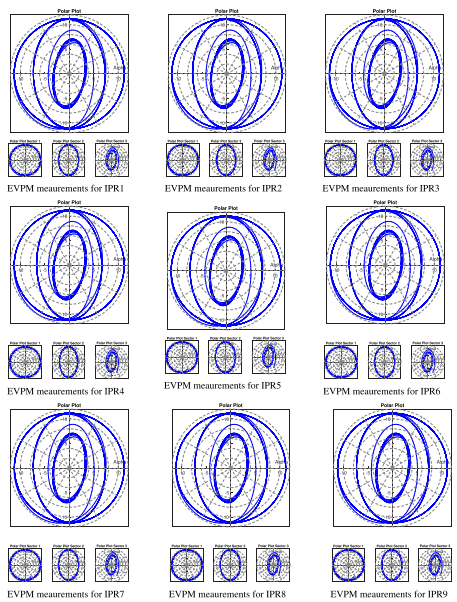
\includegraphics[width=0.75\textwidth]{images/chapter_3/SimulationCircuit2aResults.png}}
\caption{Various Case Studies.\label{Fig2}}
\end{figure}\

\begin{figure}[!ht]
\centering{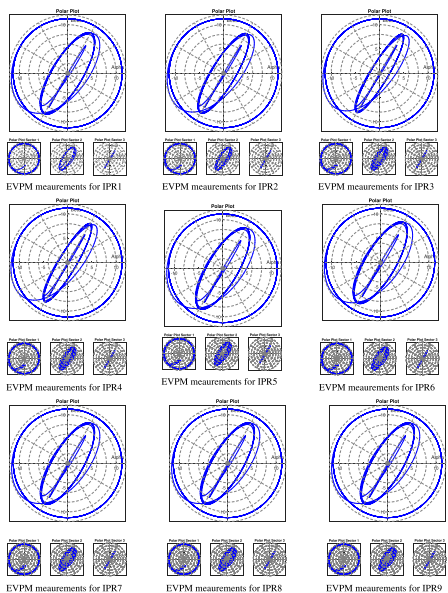
\includegraphics[width=0.75\textwidth]{images/chapter_3/SimulationCircuit2aResults2.png}}
\caption{Various Case Studies.\label{Fig2}}
\end{figure}\

\begin{figure}[!ht]
\centering{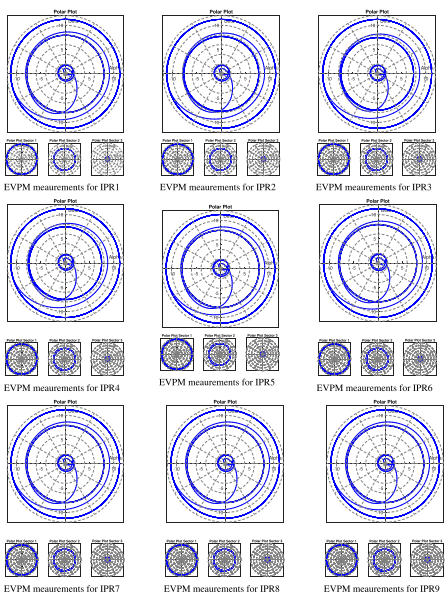
\includegraphics[width=0.75\textwidth]{images/chapter_3/SimulationCircuit2aResults3.png}}
\caption{Various Case Studies.\label{Fig2}}
\end{figure}\

\subsection{Case study 3:Evaluation of EVPM Performance in a MV distribution network with multiple DG sources}
An MV distribution network with multiple DG sources, as illustrated in Figure~\ref{Fig23}, is considered for studying  EVPM performance during various fault scenarios~\cite{pscadmvnetwork}. The distribution network operates at 20~kV, 60~Hz and is interconnected with a 230 kV high-voltage (HV) network via a 230/20~kV 100~MVA step-down transformer. The network incorporates a DFIG (Doubly Fed Induction Generator) wind farm, a PV  system, a PV battery system, and a synchronous generator with a diesel generator as the prime mover. Diverse load types are connected at buses 1, 3, and 5 as given in Figure~\ref{Fig23}.

The synchronous generator is modelled as a salient pole machine, with a rating of 13.86 kV, 2 MW, and a frequency of 60 Hz. It is driven by a diesel generator, modelled as a 12-cylinder four-stroke internal combustion engine. A governor controller is designed to regulate the power generated by the turbine. The generator field windings are connected to an exciter, which produces the magnetizing flux for the machine. The synchronous generator is connected to the grid via an interconnection transformer, which is rated at 13.86 kV/20 kV, 3 MVA.

The DFIG-based wind turbine is a variable-speed machine with a doubly-fed wound-rotor induction generator. The generator is rated at 2.5~MVA, operating at a line voltage of 0.69~kV and a frequency of 60~Hz. The wind turbine is modelled as an input torque of 0.25 pu applied to the generator. The grid-side converter and its control system regulate reactive power and DC link voltage, while the rotor-side converter and its control system regulate active and reactive power. The DFIG is integrated into the grid via an interconnection transformer rated at 0.69/20 kV, 5.5 MVA.

The PV source is modelled as a full-scale VSC operating in constant power control mode rated at 0.25 MW maximum capacity and a nominal voltage of 0.46 kV. PV array is modelled and connected to a DC-DC converter for maximum power point tracking \cite{mppttracking}. The DC-AC VSC converts it to an AC voltage with a magnitude of 0.46 kV and a frequency of 60~Hz. An LCL filter is connected to the VSC for enhanced performance. The interfacing transformer, rated at 0.5 MVA with a 0.46kV/20 kV voltage rating, connects the PV source to the distribution feeder. The controller is implemented in the dq reference frame to produce PWM reference waveforms. A limiter within the control loop restricts the maximum fault current capacity of the PV source to 1.2~pu. LVRT control is implemented, and the converter is designed to operate at unity power factor during low voltage events.

A PV source integrated with a rechargeable electrochemical battery is modelled and integrated into bus 4.~The battery is connected to a DC-DC buck-boost converter, which can operate in either buck or boost mode to charge or discharge the battery. Additionally, the PV array is integrated with a DC-DC boost converter. The output power of the PV array depends on irradiation and temperature and is kept constant during fault studies. The DC-DC converters for both the PV array and the battery are linked to a DC-AC VSC through DC link capacitors. The VSC is responsible for controlling the DC link voltage, ensuring it remains at the desired reference value, and converting it to an AC voltage of 0.46 kV at a frequency of 60 Hz. The controller operates in the dq reference frame to generate PWM reference waveforms. A limiter within the control loop restricts the maximum fault current capacity of the PV source to 1.2 per unit (PU), and the converter is designed to function at unity power factor during faults on the distribution feeder. An LCL filter is connected to the VSC for enhanced performance. An interfacing transformer, rated at 0.5 MVA with a voltage rating of 0.46 kV/20 kV, connects the VSC to the distribution feeder.

The IPRs are positioned at the PCC of all sources connected to the network, and the EVPM algorithm is incorporated. Various balanced and unbalanced fault scenarios, as mentioned in Table \ref{faultstudiescases20kV} are simulated to study the performance of the EVPM. Graphs illustrating the EVPM measurements for selected fault events are provided in the subsequent sections.

\subsubsection{Single phase to ground fault}
A single-line-to-ground fault (phase A to ground) is simulated at bus 2 during a simulation time of 5 seconds. The SPM is estimated by the EVPM using the measured three-phase voltages and projected onto the complex plane, as shown in figure~\ref{MVnetworkwithmultisources22}. Due to the fault event, the shape of the SPM changes from circular to elliptical. Figure~\ref{MVnetworkwithmultisources22} displays the segmented SPM plot for successive events estimated by their respective EVPMs. A change in the CV triggers the event flag. The type of fault is determined based on the dip type calculated from the tilt angle of the ellipse. The inclination angle shifts from \(0^\circ\) to \(89.8^\circ\), indicating a dip type of \(D_a\). The EVPM counter is activated when the CV crosses a predefined threshold, setting the fault flag. The upstream recloser opens within 0.2 seconds, and the voltage dip caused by the recloser's opening is detected at the IPR  terminals. After the recloser opens, the dip type remains unchanged, maintaining an inclination angle of \(88.2^\circ\). An instantaneous trip command is issued following the clearance of the delay counter for the first event.~All the IPRs see the same voltage sag characteristics, tripping all DG sources simultaneously, ensuring a safe reclosing condition in minimum time.

\subsubsection{Double line fault}
A line-to-line fault (phase A and phase B) was simulated at the load bus at a simulation time t = 5 seconds. The SPM in the complex plane for each EVPM at each source’s PCC is depicted in figure~\ref{MVnetworkwithmultisources22}.~Figure~\ref{MVnetworkwithmultisources22} illustrates the segmented SPM plot for successive events estimated by respective EVPMs.~The tilt angle of $59.8^o$ indicated a fault type of $C_c$ for the first event.~The upstream recloser opened within 0.2 seconds, and the voltage dip resulting from the recloser opening was sensed at the IPR terminals.~The dip type remains the same, with an inclination angle of $ 56.4^o$  after the recloser opening, and an instantaneous trip command is issued following the clearance of the delay counter for the first event.


\subsubsection{Three phase to ground fault}

A three-phase to ground fault is simulated at bus 2 with a fault impedance $1\Omega$, during simulation time t~=~5~seconds.~The estimated SPM by EVPM for each IPR at various locations is shown in Figure~\ref{MVnetworkwithmultisources22}. The SPM shape transitioned from circular of 1~pu radius to a circle of 0.3~pu radius.~The tilt angle of $0^o$ indicated a fault of type A for the first event. The upstream recloser opened within 0.2 seconds and the inclination angle remained at $0^o$ after the recloser opening.~Figure~\ref{MVnetworkwithmultisources22} illustrates the segmented SPM plot for successive events estimated by respective EVPMs.~Consistent voltage sag characteristics are observed by all IPRs, resulting in the simultaneous tripping of all sources



\begin{figure}[!ht]
\centering{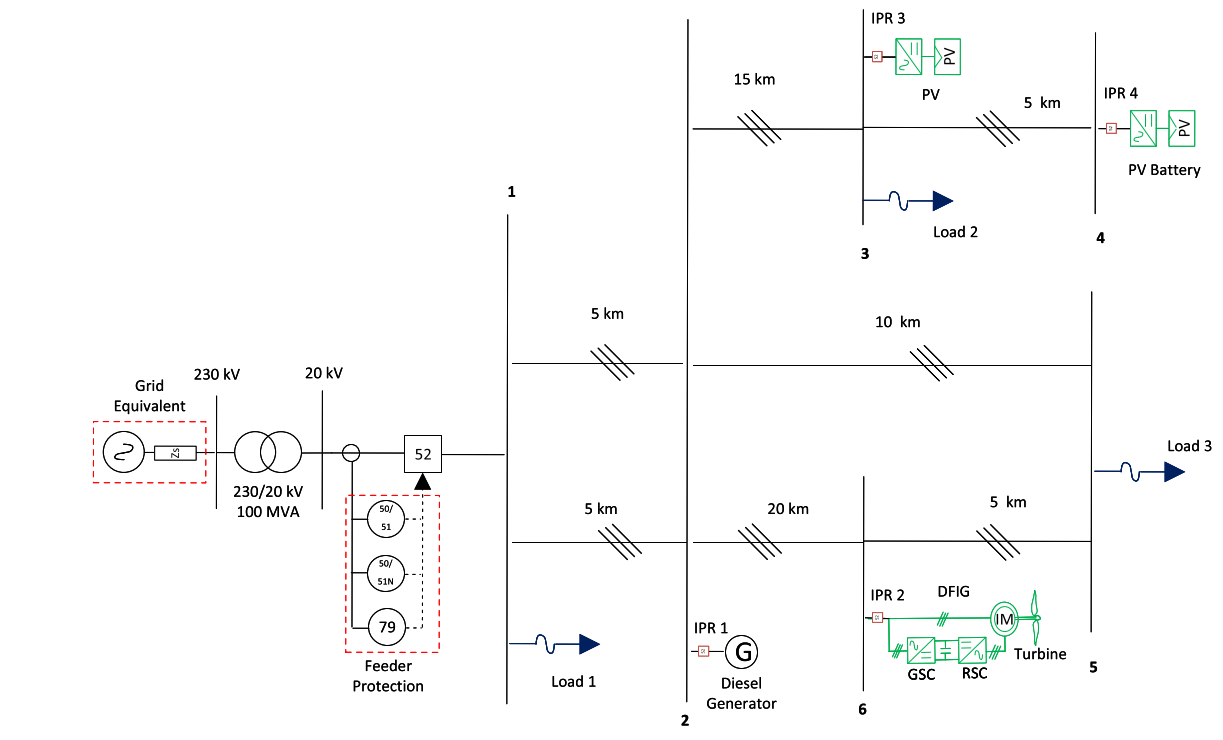
\includegraphics[width=0.75\textwidth]{images/chapter_3/SimulationCircuit3.png}}
\caption{Various Case Studies.\label{Fig2}}
\end{figure}\


\begin{figure}[!ht]
\centering{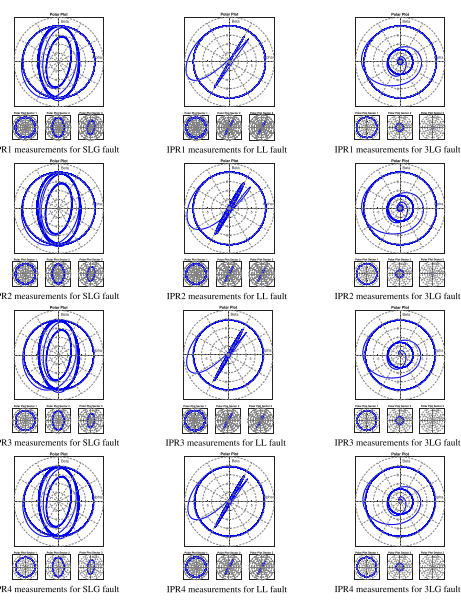
\includegraphics[width=0.75\textwidth]{images/chapter_3/SimulationCircuit3Results.png}}
\caption{Various Case Studies.\label{Fig2}}
\end{figure}\




\section{Performance evaluation of proposed advanced islanding and dynamic feature selection logics}
To validate the performance of the advanced islanding and dynamic feature selection logics, transient simulation studies were conducted using PSCAD software in three different test systems. Different undervoltage scenarios, network configurations, and operating conditions for wind power plants are studied. The results of selected cases are discussed in detail in the following sections.

Case study 1:~The test system used for case study 1 is depicted in Fig. 5. The analysis is conducted with two separate sources: one Type 3 wind plant and one Type 4 wind plant connected to the grid via switches S1 and S2. The grid is modelled as a constant voltage source with a rated voltage of 230 kV and a frequency of 50 Hz, with a system impedance (Zs) of 0.047 PU (Vbase=230 kV, Sbase=100 MVA) at the substation bus. The positive sequence line impedance for line section 1 is (0.46 + j0.47) Ohm. The Type 3 wind plant (with 100 doubly-fed induction generators (DFIGs)) is rated at 200 MW and operates at 0.69 kV.The interfacing transformer for the wind plant is rated at 200MVA and converts voltage from 0.69 kV to 33 kV in a YNd configuration. The Type 4 wind plant (with 100 permanent magnet synchronous generators (PMSG)) is also rated at 0.69 kV. The full-scale converter system is designed to decouple the PMSG from the grid, enabling variable-speed operation and precise control.A transformer rated at 200MVA and 0.69 - 33 kV, with YNd configuration interfaces the Type 4 wind plant with the grid. The wind turbine control systems are designed to optimise power extraction through maximum power point tracking (MPPT) and pitch control. The generator and grid-side converter are engineered to manage torque, flux, active/reactive power, and grid synchronisation. FRT controls are implemented in both sources to comply with grid codes. Different undervoltage scenarios and operating conditions for wind power plants are studied. The result of a selected case is given below.


Case study 2:Various simulation studies are conducted on the CIGRE benchmark system for the European medium-voltage (MV) distribution network [6] integrated with a Type 4 wind farm and a photovoltaic (PV) plant (Fig. 8). The substation transformer is three-phase 110-20 kV and 25 MVA with Dyn1 configuration, having an impedance of (0.016 + j1.92) Ohm. All line parameters and load data have been derived from reference [6]. The PV plant operates in constant power control mode and is modelled as a full-scale voltage source converter (VSC) with a maximum capacity of 5 MW and a nominal voltage of 0.65 kV. A 7.5 MVA, 0.65-20 kV YNd transformer connects the PV plant to the MV netwo. The Type 4 wind plant (modelled as done for case study 1) has a rated capacity of 18 MW and a 20MVA, 0.69/20 kV YNd transformer that interfaces with the MV network. A three-phase-to-ground fault is simulated at Bus 3 at simulation time t = 1 s and a condition where the control system of converters for different PMSG fails to operate for complying with FRT is simulated. At the wind plant terminal (Bus 8), the performance of the QDUVP application is monitored. From Fig 9, it can be observed that the Type 4 wind plant consumes the reactive power during the fault in UV conditions, and QDUVP issues the trip signal..

Case study 3:Different studies are conducted on the IEEE 39-bus benchmark system [7] integrated with a Type 3 wind plant and a Type 4 wind plant connected (one source at a time for two separate studies) at bus 19 of the benchmark system. The IEEE 39-bus benchmark system models 39 buses, 10 generators, 19 loads, and 46 transmission lines in 60Hz. The modelling of controllers for wind remains the same as in case study 1 for both wind plants. Different undervoltage scenarios and operating conditions for wind plants are studied. The results of a selected case, where a three-phase-to-ground fault and a condition where the control system of wind plants fails to operate to comply with FRT, are explained in the following section. The fault is simulated between Bus 16 and Bus 19 with a resistance of 0.1 Ohm.


\begin{figure}[!ht]
\centering{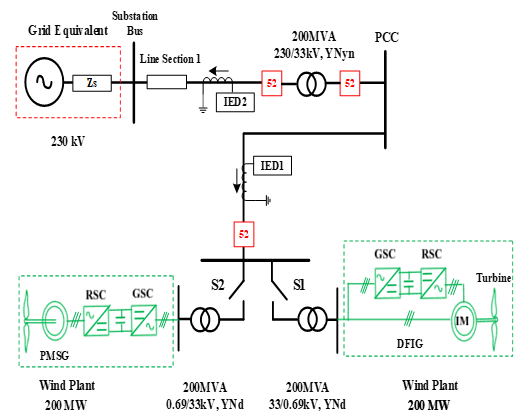
\includegraphics[width=0.75\textwidth]{images/chapter_3/Drawing2.png}}
\caption{Various Case Studies.\label{Fig2}}
\end{figure}



\begin{figure}[!ht]
\centering{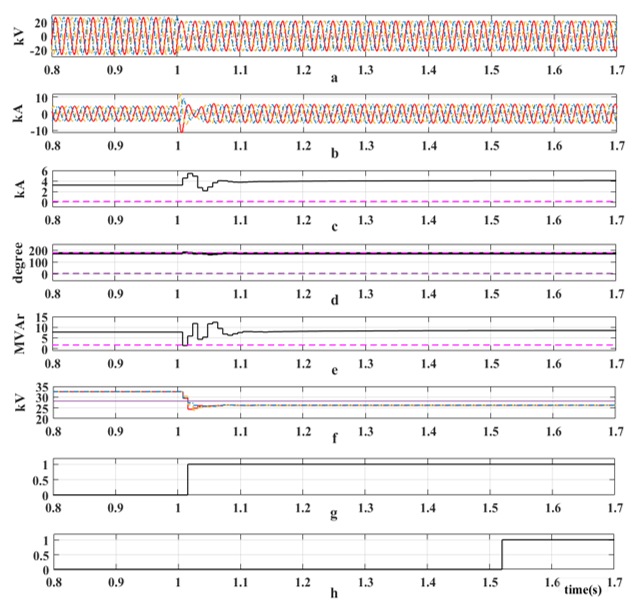
\includegraphics[width=0.75\textwidth]{images/chapter_3/Drawing4.png}}
\caption{Various Case Studies.\label{Fig2}}
\end{figure}

\begin{figure}[!ht]
\centering{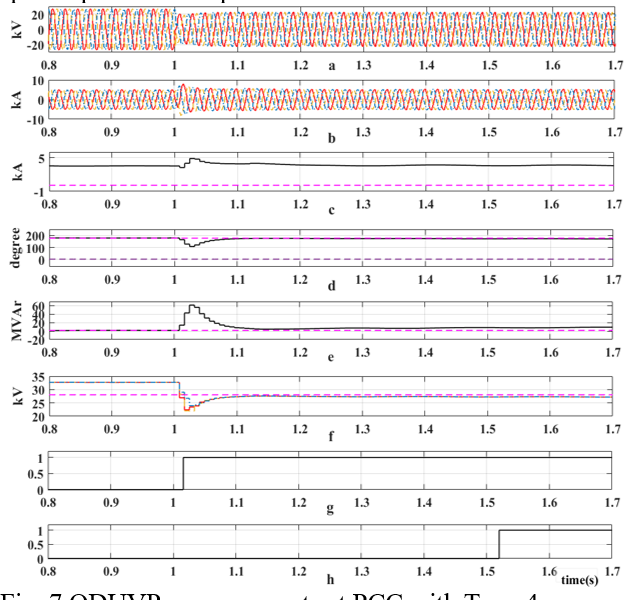
\includegraphics[width=0.75\textwidth]{images/chapter_3/Drawing5.png}}
\caption{Various Case Studies.\label{Fig2}}
\end{figure}


\begin{figure}[!ht]
\centering{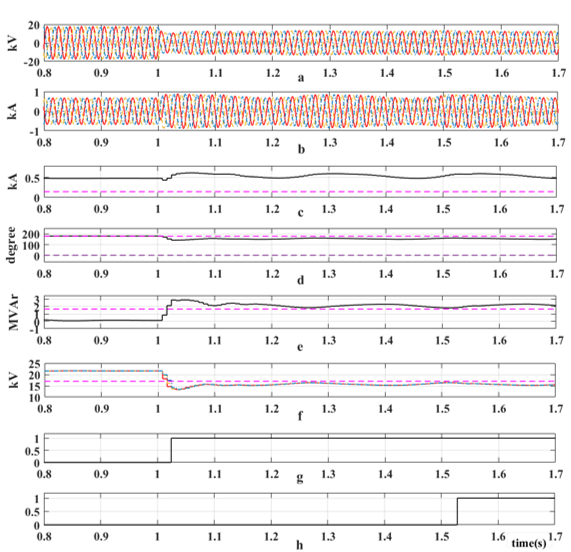
\includegraphics[width=0.75\textwidth]{images/chapter_3/Drawing6.png}}
\caption{Various Case Studies.\label{Fig2}}
\end{figure}

%\subsection{Case study 2: Evaluation of EVPM Performance in CIGRE European MV distribution network benchmark}


\begin{figure}[!ht]
\centering{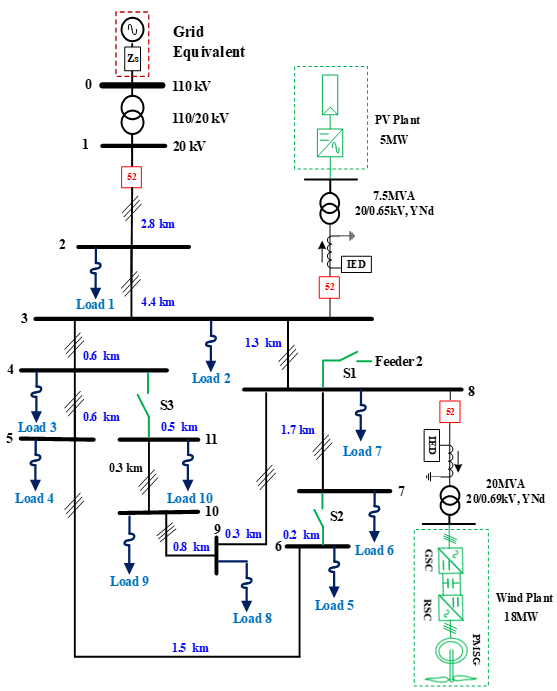
\includegraphics[width=0.75\textwidth]{images/chapter_3/Drawing3.png}}
\caption{Various Case Studies.\label{Fig2}}
\end{figure}



\begin{figure}[!ht]
\centering{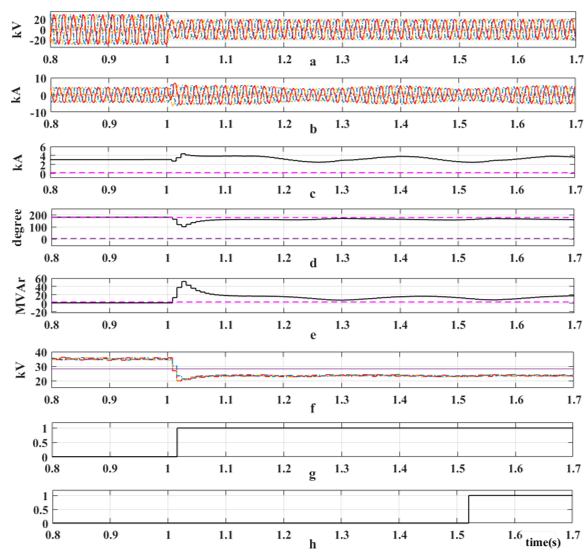
\includegraphics[width=0.75\textwidth]{images/chapter_3/Drawing7.png}}
\caption{Various Case Studies.\label{Fig2}}
\end{figure}



\begin{figure}[!ht]
\centering{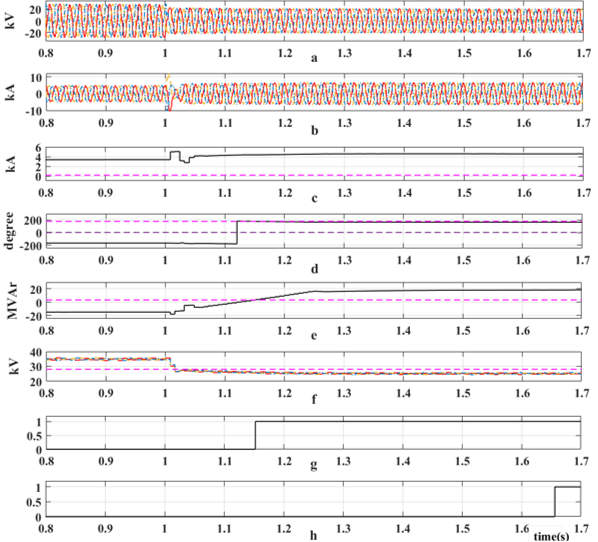
\includegraphics[width=0.75\textwidth]{images/chapter_3/Drawing8.png}}
\caption{Various Case Studies.\label{Fig2}}
\end{figure}













\section{Summary}
Interconnection protection for renewable and distributed generation (DG) is essential for ensuring the stability and reliability of the power grid as more renewable energy sources, such as solar and wind, are integrated.The primary goal of interconnection protection is to safeguard both the distributed generation units and the grid. It ensures that DG units can operate in parallel with the grid without causing instability or damage. Previously DG units have been required to be disconnected during utility grid faults /islanding situations, Based on voltage, frequency, rate-of-change-frequency or vector shift, Without any specific requirements to support utility grid (HV Network).

Advanced interconnection protection systems can keep DG units connected during minor disturbances, helping to maintain grid stability and reliability ~\cite{rantzer2009dynamic}.Modern protection systems often use communication-based schemes to coordinate between the DG units and the grid, ensuring timely and accurate responses to faults~\cite{terelius2011decentralized}.
 

